%%%%%%%%%%%%%%%%%%%%%%%%%%%%%%%%%%%%%%%%%%%%%%%%%
%% Parametrization
%%%%%%%%%%%%%%%%%%%%%%%%%%%%%%%%%%%%%%%%%%%%%%%%%
\def\lang{EN} % The language: CZ = Czech, EN = English

\def\faculty{Faculty of Electrical Engineering} % Full faculty/or institute name 
\def\department{Department of Control Engineering} % Full name of the department

\def\worktype{Bachelor's thesis}  % Type: Bachelor's thesis, Master's thesis, ...
\def\title{Development of RC car controlled by STM32 microcontrollers} % Thesis name
\def\subtitle{} % Optional subtitle

\def\author{Kristi\'{a}n \v{S}lehofer} % Name of the author
\def\date{May 2022} % Date 

\def\supervisor{Ing. Jan Stejskal} % Supervisor name
\def\supervisorspecialist{} % Optional name of supervisor specialist

%%%%%%%%%%%%%%%%%%%%%%%%%%%%%%%%%%%%%%%%%%%%%%%%%
%% Document class
%%%%%%%%%%%%%%%%%%%%%%%%%%%%%%%%%%%%%%%%%%%%%%%%%
\documentclass[11pt,a4paper,twoside]{CTUthesis}
\usepackage[utf8]{inputenc}

%%%%%%%%%%%%%%%%%%%%%%%%%%%%%%%%%%%%%%%%%%%%%%%%%
%% User packages
%%%%%%%%%%%%%%%%%%%%%%%%%%%%%%%%%%%%%%%%%%%%%%%%%
\usepackage{times} % times font
\usepackage{amsmath}
\usepackage{amssymb}
\usepackage{subcaption}
\usepackage{cite}
%\usepackage[anythingbreaks]{breakurl}
\usepackage{url}
\usepackage{mathtools, nccmath}
\usepackage{array}
\usepackage{tabularx}
\usepackage{multirow}

\usepackage{booktabs}

\usepackage{pdfpages}

\usepackage{tablefootnote} % for table footnotes
\usepackage{xurl}	% for too long urls
\usepackage{siunitx}	
	\DeclareSIUnit{\Kv}{Kv}
\usepackage{bytefield}
\usepackage[square,numbers]{natbib}

\usepackage[edges]{forest} % for directory tree, https://tex.stackexchange.com/questions/328886/making-a-directory-tree-of-folders-and-files/328987#328987, https://tex.stackexchange.com/questions/405192/how-to-insert-folder-icon-in-root-node-with-forest-package/405253#405253
\definecolor{folderbg}{RGB}{124,166,198}
\definecolor{folderborder}{RGB}{110,144,169}
\newlength\Size
\setlength\Size{4pt}
\tikzset{%
  folder/.pic={%
    \filldraw [draw=folderborder, top color=folderbg!50, bottom color=folderbg] (-1.05*\Size,0.2\Size+5pt) rectangle ++(.75*\Size,-0.2\Size-5pt);
    \filldraw [draw=folderborder, top color=folderbg!50, bottom color=folderbg] (-1.15*\Size,-\Size) rectangle (1.15*\Size,\Size);
  },
  file/.pic={%
    \filldraw [draw=folderborder, top color=folderbg!5, bottom color=folderbg!10] (-\Size,.4*\Size+5pt) coordinate (a) |- (\Size,-1.2*\Size) coordinate (b) -- ++(0,1.6*\Size) coordinate (c) -- ++(-5pt,5pt) coordinate (d) -- cycle (d) |- (c) ;
  },
}
\forestset{%
  declare autowrapped toks={pic me}{},
  declare boolean register={pic root},
  pic root=1,
  pic dir tree/.style={%
    for tree={%
      folder,
      font=\ttfamily,
      grow'=0,
      s sep=0.5mm, inner sep=3
    },
    before typesetting nodes={%
      for tree={%
        edge label+/.option={pic me},
      },
      if pic root={
        tikz+={
          \pic at ([xshift=\Size].west) {folder};
        },
        align={l}
      }{},
    },
  },
  pic me set/.code n args=2{%
    \forestset{%
      #1/.style={%
        inner xsep=2\Size,
        pic me={pic {#2}},
      }
    }
  },
  pic me set={directory}{folder},
  pic me set={file}{file},
}

\newlength\mystoreparindent
\newenvironment{myparindent}[1]{%
\setlength{\mystoreparindent}{\the\parindent}
\setlength{\parindent}{#1}
}{%
\setlength{\parindent}{\mystoreparindent}
}


%%%%%%%%%%%%%%%%%%%%%%%%%%%%%%%%%%%%%%%%%%%%%%%%%
% MY COMMANDS
%%%%%%%%%%%%%%%%%%%%%%%%%%%%%%%%%%%%%%%%%%%%%%%%%
\usepackage{xspace}
%\usepackage[T1]{fontenc}

\newcommand{\disable}[1]{}

\newcommand{\revise}[1]{{\color{blue}#1}}
\newcommand{\rewrite}[1]{{\color{red}#1}}
\newcommand{\todo}[1]{{\color{red}\colorbox{yellow}{\textbf{TODO:}}\color{red}#1}}

% improved colomns
\newcolumntype{L}[1]{>{\raggedright\let\newline\\\arraybackslash\hspace{0pt}}m{#1}}
\newcolumntype{C}[1]{>{\centering\let\newline\\\arraybackslash\hspace{0pt}}m{#1}}
\newcolumntype{R}[1]{>{\raggedleft\let\newline\\\arraybackslash\hspace{0pt}}m{#1}}

% improved cline
%\newlength{\Oldarrayrulewidth}
%\newcommand{\Cline}[2]{%
%  \noalign{\global\setlength{\Oldarrayrulewidth}{\arrayrulewidth}}%
%  \noalign{\global\setlength{\arrayrulewidth}{#1}}\cline{#2}%
%  \noalign{\global\setlength{\arrayrulewidth}{\Oldarrayrulewidth}}}

\begin{document}
%%%%%%%%%%%%%%%%%%%%%%%%%%%%%%%%%%%%%%%%%%%%%%%%%
%% Document head
%%%%%%%%%%%%%%%%%%%%%%%%%%%%%%%%%%%%%%%%%%%%%%%%%
\TitlePage
%\setboolean{@twoside}{false}

%% thesis assignment %%%%%%%%%%%%%%%%%%%%%%%%%%%%%%%%%%%%
\newpage\null\thispagestyle{empty}\newpage\addtocounter{page}{-1}
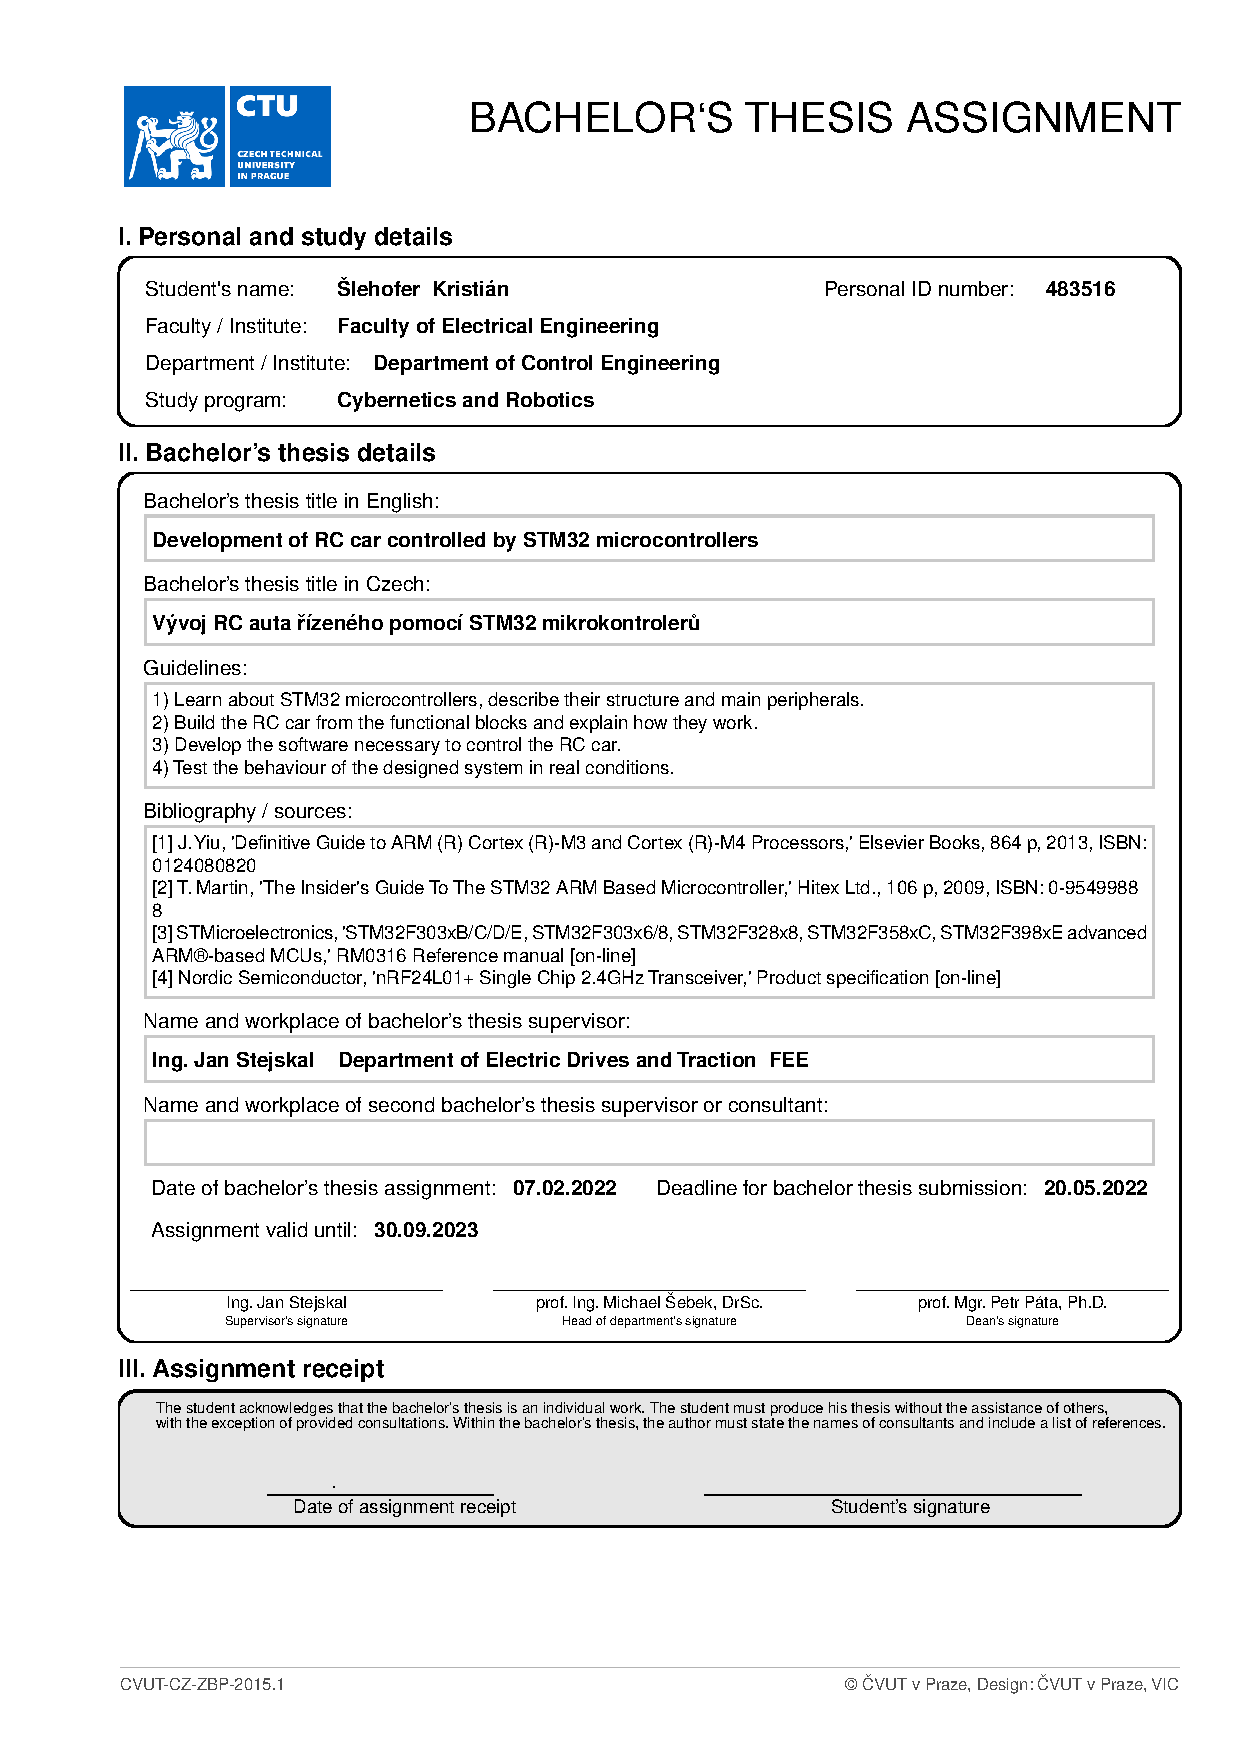
\includepdf[pages=-, offset=+11 0]{src/Thesis_Assignment.pdf}

\begin{document_head}
%% declaration, acknowledgement, abstract %%%%%%%%%%%%%%%
	\newpage
	\null\vfill{}
%\section*{Prohlášení}
\section*{Declaration}
I declare that the presented work was developed independently ant that I have listed all sources of the information used within it in accordance with the methodical instructions for observing the ethiclal principles in the preparation of university theses.\\[0.5cm]

Prague, May 20, 2022	
\bigskip
\bigskip
\bigskip 

\begin{flushright}  

 \begin{minipage}{0.35\textwidth} 
  \centering   
  \dotfill\\   
  Kristián Šlehofer
 \end{minipage}
\end{flushright}
	\newpage
	%\null \vfill{}
%\section*{Poděkování}
%poděkování...\\
%
%\section*{Acknowledgement}
%Thanks...\\
\null \vfill{}
\section*{Acknowledgement}

I would like to thank ...
	\newpage
	\section*{Abstract}
\vspace{0.5cm}

This thesis focuses on building a radio-controlled car powered by STM32 microcontrollers. It describes the development of both the car and transmitter, presents hardware parts and their utilization, and explains the control software in detail.

The controlling system was developed from scratch on top of an old Tamiya chassis and consists of a custom-made control board with modules and necessary control software. The chassis was modified and equipped with more powerful BLDC motor. In order to retrofit the transmitter, a custom PCB was designed. In addition to the essential functions, the car features various sensors and modules with the ability to log the data to the micro SD card. Also, the car status is reported back to the transmitter and visualized on an OLED display.

The developed RC system is tested in real conditions at the end of the thesis. Besides, the maximum controllable range and top speed are measured.

\vspace{1cm}
\noindent{\bf Keywords:} STM32, RC car, control software, embedded system, retrofitting

	\newpage
	\section*{Abstrakt}
\vspace{0.5cm}

Tato práce se zaměřuje na vývoj auta na dálkové ovládání poháněného STM32 mikrokontroléry. Popisuje stavbu jak auta, tak i vysílačky, představuje použité hardwarové části a jejich využití a~podrobně vysvětluje řídicí software.

Řídicí systém byl od základu vyvinut na starém podvozku Tamiya a tvoří ho na míru vyrobená ovládací deska s moduly a nezbytný řídicí software. Podvozek byl upraven a vybaven výkonnějším BLDC motorem. Aby bylo možné modernizovat vysílačku, byla navržená vlastní deska plošných spojů. Kromě základních funkcí je vůz vybaven různými senzory a moduly s~možností záznamu dat na micro SD kartu. Stav vozu je také nahlašován zpět do vysílačky a~zobrazován na OLED displeji.

Vyvinutý RC systém je v závěru práce otestován v reálných podmínkách. Kromě toho je změřen maximální kontrolovatelný dosah a maximální rychlost.

\vspace{1cm}
\noindent{\bf Klíčová slova:} STM32, RC auto, řídicí software, vestavěný systém, retrofitting

\noindent{\bf Překlad názvu:} Vývoj RC auta řízeného pomocí STM32 mikrokontrolerů

	\newpage
	
%% table of contents %%%%%%%%%%%%%%%%%%%%%%%%%%%%%%%%%%%%
	\tableofcontents
	\newpage
%% list of figures %%%%%%%%%%%%%%%%%%%%%%%%%%%%%%%%%%%%%%	
	\listoffigures
	\newpage
%% list of tables %%%%%%%%%%%%%%%%%%%%%%%%%%%%%%%%%%%%%%%	
	\listoftables
	\newpage
%% list of listings %%%%%%%%%%%%%%%%%%%%%%%%%%%%%%%%%%%%%	
%	\listoflistings
%% list of abbreviations
	\section*{List of Abbreviations}
\begin{table}[h]
   \renewcommand{\arraystretch}{1.1}
   \centering
%    \caption{ARM Core utilization in STM32 family}
    \label{tab:abbrev}   
    \begin{tabular}{c c}
       \noalign{\hrule height 1.1pt}\noalign{\smallskip}
	   \bfseries Abbreviation & \bfseries Meaning\\[0.2em]
	\noalign{\hrule height 1.1pt}\noalign{\smallskip}  

API		& Application Programming Interface \\
ACK		& Acknowledgment packet \\ 
ADC		& Analog-to-Digital Converter \\
AHB		& Advanced High-performance Bus \\
APB		& Advanced Peripheral Bus \\
AXI		& Advanced eXtensible Interface \\
BEC		& Battery Eliminator Circuit \\
BLDC		& Brushless DC electric motor \\
CAD		& Computer-Aided Design \\
CRC		& Cyclic Redundancy Check \\
DAC		& Digital-to-Analog Converter \\
DIP		& Dual In-line Package \\
DMA		& Direct Memory Access \\
DSP		& Digital Signal Processor \\
EPROM	& Erasable Programmable Read-Only Memory \\
ESC		& Electronic Speed Controller \\
%EXTI		& External Interrupt/event controller \\		% jednou
FPU		& Floating Point Unit \\
GPIO		& General-Purpose Input/Output \\
I\textsuperscript{2}C	& Inter-Integrated Circuit \\
IMU		& Inertial Measurement Unit \\
LiPo		& Lithium-ion Polymer battery \\
MCU		& Microcontroller Unit \\
%MPU		& Memory Protection Unit \\					% jednou
Ni-Cd	& Nickel-Cadmium battery \\
%NMI		& Non-Maskable Interrupt \\					% jednou
NVIC		& Nested Vectored Interrupt Controller \\	% 3x v jedne sekci
OLED		& Organic Light-Emitting Diode (display type) \\
%OS		& Operating System \\
PCB		& Printed Circuit Board \\
%PLL		& Phase-Locked Loop \\						% jednou
PWM		& Pulse Width Modulation \\
RC		& Radio Control \\ 
SDRAM	& Synchronous Dynamic Random Access Memory \\
SPI		& Serial Peripheral Interface \\
SRAM		& Static Random Access Memory \\
UART		& Universal Asynchronous Receiver and Transmitter \\
%VBAT		& pin for connecting external battery \\
VDDA		& Analog supply voltage pin \\




% ??? AC, DC, USB, TCP/IP, VBAT
       \noalign{\smallskip}\noalign{\hrule height 1.1pt}
    \end{tabular}
\end{table} 

%% for printing purposes it is possible to use this line between individual inputs to achieve all-double page printing
%\newpage\null\thispagestyle{empty}\newpage\addtocounter{page}{-1}
\end{document_head}

%%%%%%%%%%%%%%%%%%%%%%%%%%%%%%%%%%%%%%%%%%%%%%%%%
%% Document body
%%%%%%%%%%%%%%%%%%%%%%%%%%%%%%%%%%%%%%%%%%%%%%%%%
\begin{document_body}
  	
%!TEX ROOT=slehokri_bp.tex

\chapter{Introduction}
\label{chap:intro}
%TODO

\section{Motivation}
%TODO





	\clearpage
%	\newpage\null\thispagestyle{empty}\newpage\addtocounter{page}{-1}
	
%!TEX ROOT=main.tex


\part{STM32 microcontrollers}
\label{chap:STM}
\section{Indroduction}
\label{sec:stm_intro}
STM32 is a family of 32-bit microcontrollers by STMicroelectronics based on ARM Cortex-M processor, namely Cortex-M3, Cortex-M4(F), Cortex-M0, Cortex-M0+, Cortex-M7F, and Cortex-M33F. The STM32 family consists of numerous series of microcontrollers designed for various use-cases. These can be divided into four main groups: Mainstream, High Performance, Ultra-low-power, and Wireless series. As every series has specific features and peripherals, this section will only focus on the main differences between used ARM Cortex cores. Table \ref{tab:cortex} shows the utilization of ARM cores in the particular STM32 series.
%\begin{table}[ht]
%\begin{ctucolortab}
%\begin{tabular}{cc}
%\bfseries ARM Core & \bfseries STM32 series \\\Midrule
%Cortex-M3 & F1, F2, L1 \\ 
%Cortex-M4F & F3, F4, G4, L4, L4+, WB, WL\tablefootnote{Based only on ARM Cortex-M4 (without FPU).} \\	
%Cortex-M0 & F0 \\ 
%Cortex-M0+ & G0, L0 \\
%Cortex-M7F & F7, H7 \\
%Cortex-M33F & L5, U5
%\end{tabular}
%\end{ctucolortab}
%\caption{ARM Core utilization in STM32 family}
%\label{tab:cortex}
%\end{table}

\begin{table}[ht]
   \renewcommand{\arraystretch}{1.1}
   \centering
    \caption{ARM Core utilization in STM32 family}\label{tab:cortex}   
    \begin{tabular}{c c}
       \noalign{\hrule height 1.1pt}\noalign{\smallskip}
	   \bfseries ARM Core & \bfseries STM32 series\\[0.2em]
	\noalign{\hrule height 1.1pt}\noalign{\smallskip}     
Cortex-M3 & F1, F2, L1 \\ 
Cortex-M4F & F3, F4, G4, L4, L4+, WB, WL\tablefootnote{Based only on ARM Cortex-M4 (without FPU).} \\	
Cortex-M0 & F0 \\ 
Cortex-M0+ & G0, L0 \\
Cortex-M7F & F7, H7 \\
Cortex-M33F & L5, U5 \\
       \noalign{\smallskip}\noalign{\hrule height 1.1pt}
    \end{tabular}
\end{table} 

\section{Division by ARM cores}
\label{sec:stm_arm_division}
	\subsection{Cortex-M3}
	\label{sub:stm_m3}
Cortex-M3 was the first processor in the Cortex-M generation and the first core used in the STM32 family in the STM32F1 series of microcontrollers. ARM first released this high-performance processor based on ARMv7-M architecture in 2005. It features modified Harvard architecture (with unified memory space) and a 3-stage pipeline. Thanks to 32-bit addressing, 4GB of memory space is supported.
	
	\subsection{Cortex-M4F}
	\label{sub:stm_m4}
The successor to Cortex-M3 was released by ARM in 2010. This new generation called Cortex-M4 is similar to its predecessor in design and features. The instruction set now contains DSP (Digital Signal Processor) instructions for more complex data processing, and there is an optional single-precision FPU (Floating Point Unit). Variant with FPU is known as Cortex-M4F. 
	
	\subsection{Cortex-M0}
	\label{sub:stm_m0}		%TODO citace?
Cortex-M0 processor is one of the smallest ARM processors available, optimized for small size and low power consumption \cite{m0_web}. The processor is based on ARMv6-M with a smaller instruction set, uses Von Neumann architecture, and has a 3-stage pipeline. This small core is ideal for general data processing tasks, where low cost and high energy efficiency matter.
	
	\subsection{Cortex-M0+}
	\label{sub:stm_m0_plus}
Cortex-M0+ is based on Cortex-M0, thus adopting small a size and further improving power efficiency and performance. The instruction set and tools are fully backward compatible with Cortex-M0. ARM reduced pipeline to 2 stages to lower power consumption. Furthermore, the processor has more options available, such as vector table relocation and memory protection unit (MPU).
	
	\subsection{Cortex-M7F}
	\label{sub:stm_m7}
The most powerful processor in the Cortex-M family is Cortex-M7. The processor uses ARMv7-M architecture and features the longest pipeline with six stages. Given the used architecture, the instruction set contains DSP instructions, and there is also an optional FPU, which can be single-precision or even double-precision. Main buses have been enlarged to 64-bit wide. Variant with FPU is known as Cortex-M7F. 
	
	\subsection{Cortex-M33F}
	\label{sub:stm_m33}
Cortex-M33 is the newest core used in the STM32 family of microcontrollers. The processor is based on more recent ARMv8-M architecture with Harvard bus architecture. It is conceptually similar to Cortex-M4 with a 3-stage pipeline and optional single-precision FPU. The core is ideal for IoT applications as it has optional TrustZone security instructions for hardware-enforced isolation and memory protection unit (MPU). Variant with FPU is known as Cortex-M33F. 

\section{Architecture}
\label{sec:stm_arch}
ARM as a company does not construct microcontrollers but instead designs the core and other components and licenses them to silicon designers. It is the same concept with the STM32 family of microcontrollers - ST Microelectronics obtains the processor design from ARM as a base for their microcontroller. The company then attaches its own set of memories and peripherals, such as ADC (Analog-to-Digital converter), DAC (Digital-to-Analog converter), clock generation and timers, and various types of connectivity peripherals like UART, SPI, I2C, etc.

This approach is illustrated in figure \ref{fig:f303}, which shows the circuit diagram of the STM32F303CC microcontroller used in this project. It shows the Cortex-M4F processor with all the ST-specific peripherals and memories around.
\begin{figure}
\centering
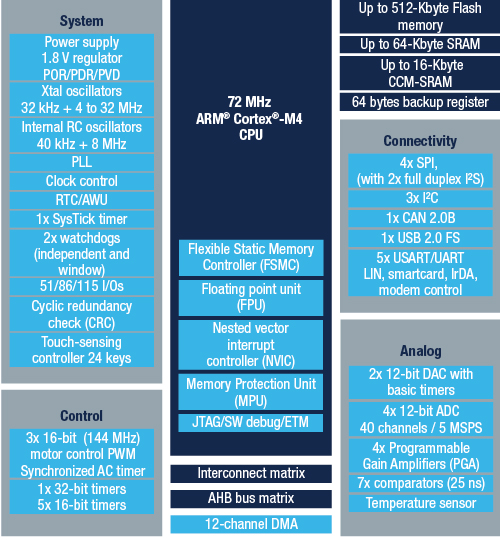
\includegraphics[width=0.6\linewidth]{support/pic/en.bd_stm32f303.jpg}
\caption{STM32F303 circuit diagram \cite{f303_diagram}} %TODO citace - web ST
\label{fig:f303}
\end{figure}

	\subsection{Clock}
	\label{sub:clock}
The frequency of the processor, buses, and connected peripherals is derived from their clock source, usually an oscillator. STM32 microcontrollers include internal clock sources, or it is possible to connect external clock sources. The frequency from other clock sources can be multiplied by the internal PLL (Phase-Locked Loop) circuit to speed up the microcontroller further and reach higher frequencies. Several prescalers allow finetuning bus and peripherals speed. Internal clock sources have the advantage of providing a clock source at a low cost with no external components. However, being an RC oscillator, the frequency produced is usually not as accurate as an external oscillator.

	\subsection{Interrupts}
	\label{sub:nvic}
The main controller responsible for handling interrupt events is Nested Vectored Interrupt Controller, NVIC for short. It is tightly coupled to the Cortex core allowing for low latency interrupt processing. The NVIC features support for up to 240 interrupt inputs with programmable priorities, which can be individually enabled or disabled, along with Non-Maskable Interrupts (NMI). Furthermore, in the case of Cortex M3 and M4, the interrupt latency is only 12 cycles with zero wait state memory \cite{yu}. All interrupts can be triggered by software by writing to the appropriate register; this also applies to many system exceptions. Microcontroller vendors determine the total number of interrupts supported by the device with Cortex core when designing the chip.

In the  STM32 family of microcontrollers, there is also a hardware device called extended interrupts and events controller (EXTI). This controller is connected to the NVIC and supports up to 36 external/internal interrupt events. Active edge for external interrupts is programmable. This device makes it possible to generate interrupts or wake-up events from external peripherals and GPIO pins.

	\subsection{Buses}
	\label{sub:buses}
The Cortex core has a well-defined on-chip bus structure and protocol that allows the connection of various memory configurations and peripherals. Since most of the Cortex cores use Harvard architecture, multiple bus interfaces enable simultaneous access to instructions and data. Buses are (most of the time) 32-bit wide.

The primary bus interface protocol utilized is AHB Lite (Advanced High-performance Bus). This pipelined protocol allows high operation frequency with a small silicon footprint and is used in program memory and system bus interfaces. Usually, the bus can have more devices that act as a master, for example, DMA (Direct Memory Acces) or Ethernet controller. Therefore the processor includes a bus matrix (or AHB interconnect matrix) that manages transfers from multiple bus masters to different slave segments. Particular bus matrix implementation is shown in figure \ref{fig:f303_busmatrix}.
\begin{figure}
\centering
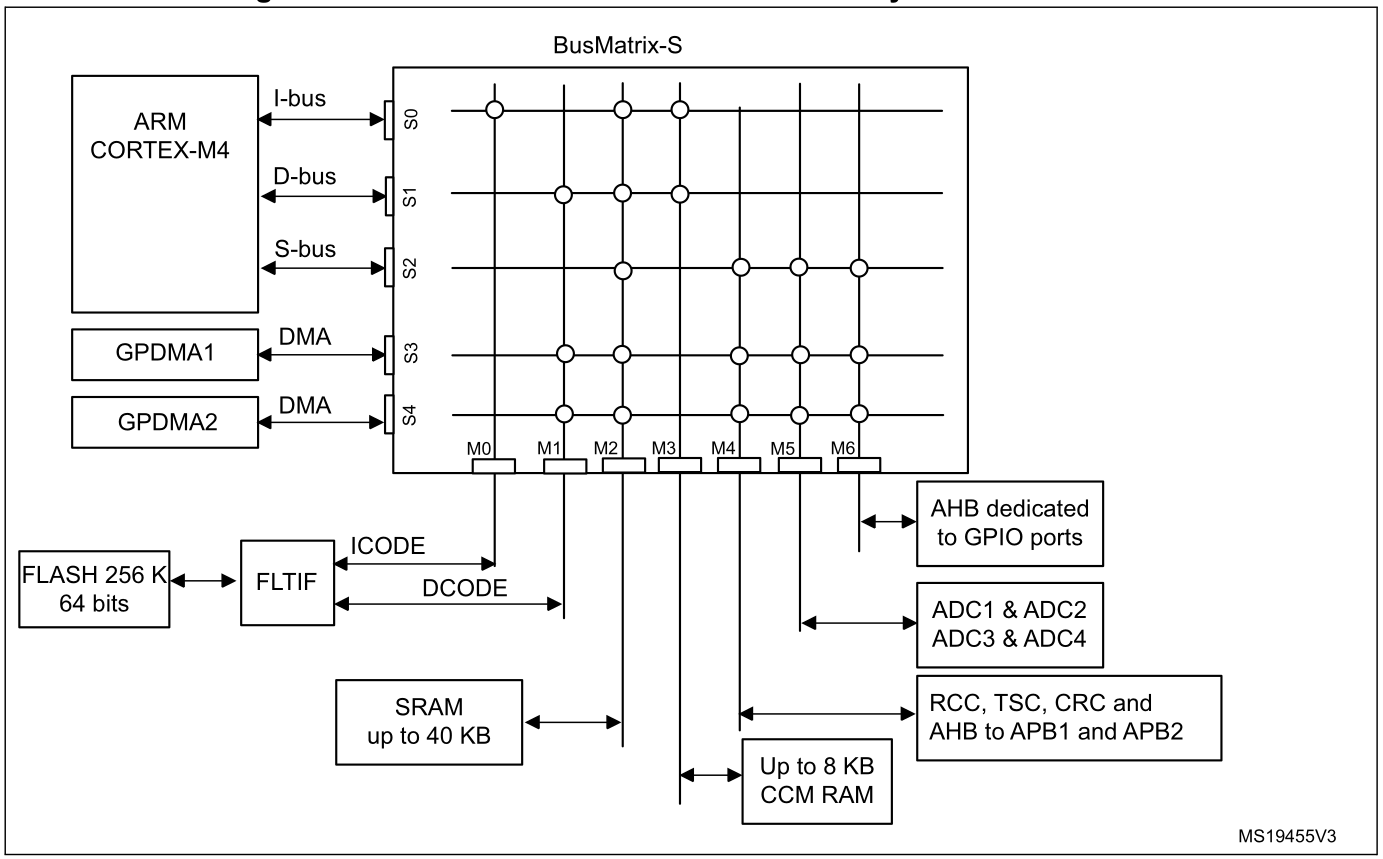
\includegraphics[width=0.7\linewidth]{support/pic/f303_bus_matrix.png}
\caption{STM32F303CC bus architecture \cite{f303_ref}} %TODO citace - referencak F303
\label{fig:f303_busmatrix}
\end{figure}

The secondary bus used mainly for connecting peripherals is APB (Advanced Peripheral Bus). Usually, APB buses are connected to the AHB bus matrix using bridge components. If the peripheral needs higher bandwidth and operation speed, for example, the ADC, it is possible to connect it to the faster AHB bus.

Some of the more advanced Cortex processors also use other buses. For example, the Cortex-M7 has an additional 64-bit wide AXI bus that can be used for faster FLASH memory access. 

	\subsection{Memories}
	\label{sub:memories}
Thanks to the bus architecture, different memories can easily be attached to the AHB bus with suitable memory interface logic. Even though the bus is 32-bit, there are no width restrictions if appropriate conversion hardware is used.

Usually, types like SRAM and FLASH are often used for data memory and program code memory, respectively. However, there is no real limitation on memory type connected to a processor, and different technologies can be utilized, e.g., SDRAM, EPROM, etc. Also, memory size is not limited. The only requirement is that the memory should be byte-addressable, and the interface has to support byte, half-word, and word transfers.

	\subsection{Direct Memory Acces (DMA)}
	\label{sub:dma}
A Direct Memory Access is a programmable hardware unit connected to the AHB bus. It reduces processor load by offloading memory transfer operations. Supported transfer directions are peripheral-to-peripheral, memory-to-peripheral, peripheral-to-memory, and also memory-to-memory. There is a small overhead when setting the unit, but afterward, the whole transfer is handled by DMA without processor intervention, thus leaving computing power to other tasks. The unit usually has several independent channels with assignable priorities.


\section{Peripherals}
\label{sec:stm_periph}
Every series of STM32 microcontrollers features different peripherals, from the basic ones with little settings to more advanced and configurable ones. This section is not supposed to be an overly exhausting listing of all the peripherals across all STM32 families, but instead, it focuses mainly on the most used ones and those used in this project.

	\subsection{GPIO}
	\label{sub:gpio}
The abbreviation GPIO stands for General-Purpose Input/Output. It is a designation for microcontroller pins. The pins are arranged in groups of sixteen and are referred to as GPIOx (for example, GPIOA, GPIOC). Not every pin from the group has to be physically present. Especially for microcontrollers with smaller packages, it is usual that some pins from the group are missing. In figure \ref{fig:gpio}, there is a typical internal structure of the GPIO pin with internal protection diodes.

Each pin can be set as either input, output, or alternate function. Internal pull-up and pull-down resistors are available as well. These features are configured and controlled by software. Most GPIO control registers are 32-bit and have to be accessed as 32-bit words, although some STM32 series support half-word and byte access.

If the pin is in alternate function mode, it is controlled by a connected peripheral, for example, ADC, timer, or USART. Thanks to the highly flexible pin multiplexing, many peripheral functions can be remapped to another pin. Debug pins are in alternate function mode by default after microcontroller reset. Other pins are usually in floating input mode.

When the pin is set as output or alternate function, it can be push-pull or open-drain. Most of the pins can provide $\pm20 \text{ mA}$ of current, making it possible to drive, for example, a LED directly. However, the total current that a microcontroller can source or sink is limited. Connecting pins to voltages higher than the supply voltage is not recommended, yet many pins are 5V tolerant.
\begin{figure}
\centering
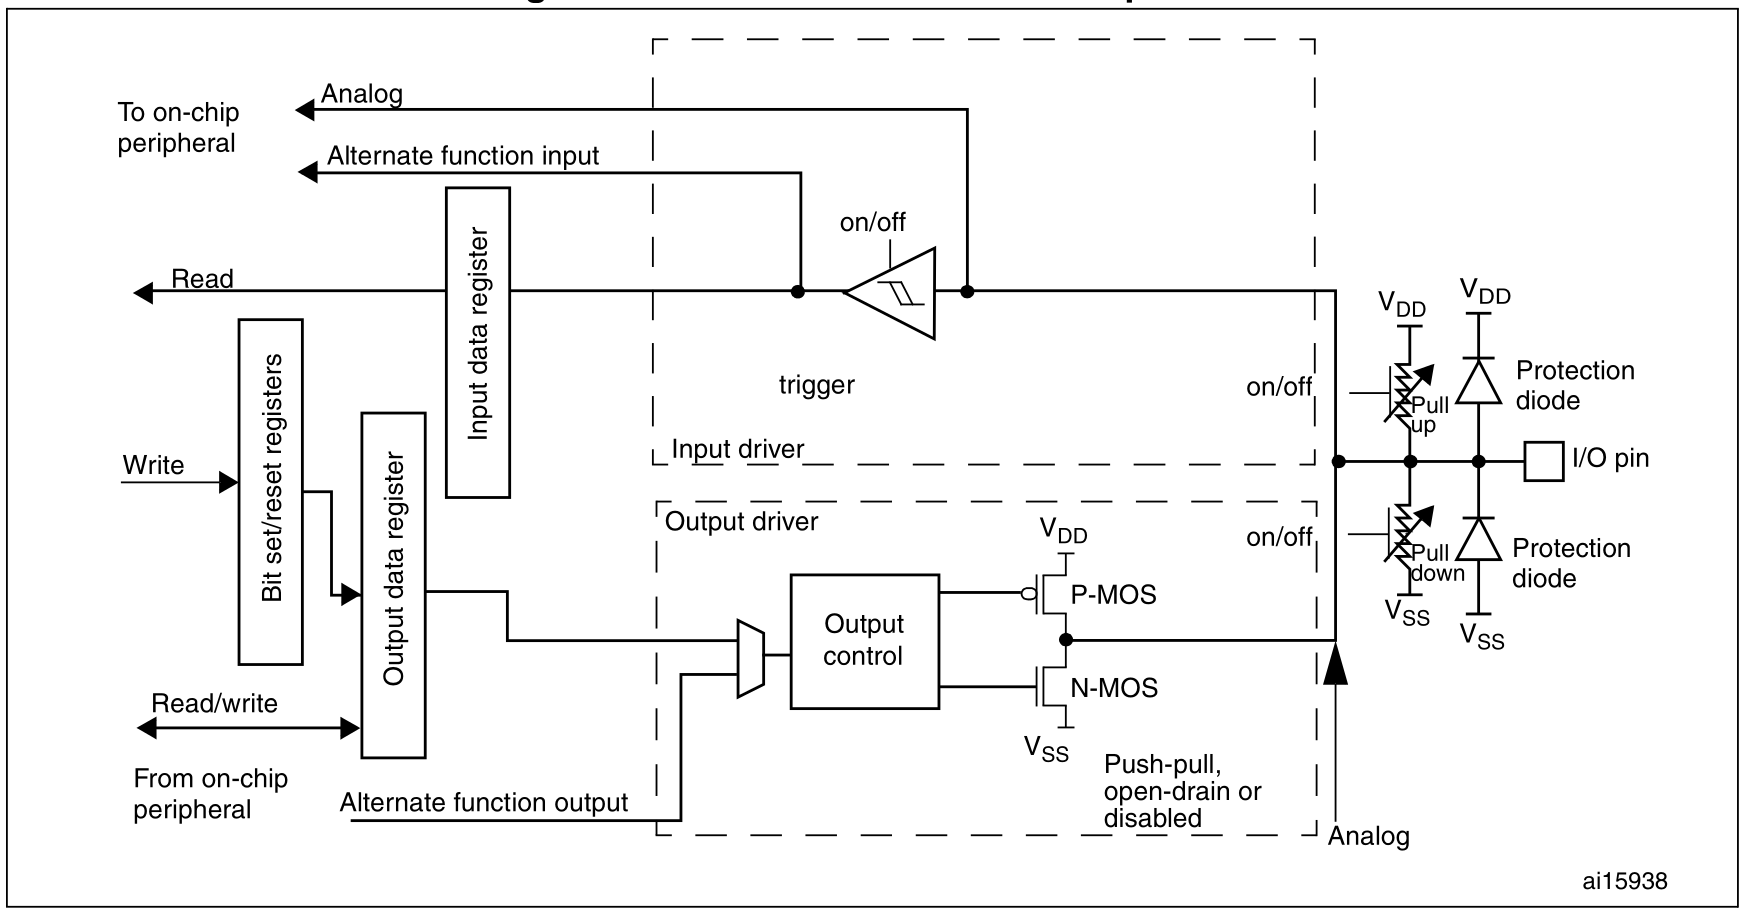
\includegraphics[width=0.9\linewidth]{support/pic/io_port.png}
\caption{Basic structure of an I/O port bit \cite{f303_ref}} %TODO citace - referencak F303
\label{fig:gpio}
\end{figure}

	\subsection{Timers}
	\label{sub:timers}
Timers are one of the basic peripherals. The primary function is counting; it can measure time and do a specific action, for example, toggle a pin. The counter clock frequency is adjustable using a programmable prescaler. Usually, there are many timers in the microcontroller with varying features.

The simplest ones are basic timers. These timers are predominantly used for time-base generation as they feature only a simple up counter, usually 16-bit.

The more feature-rich timers are general-purpose timers. With those, besides the basic functionality, it is possible to generate various waveforms or measure the pulse length of the input signal. Furthermore, there can be support for incremental encoders with quadrature output, which can then be connected straight to the MCU. This feature is handy and makes interfacing encoders pretty straightforward.

As the name suggests, the advanced-control timers are the most advanced. Functionality includes all the features of previously mentioned timers with some added or upgraded. Most of the time, advanced-control timers have more channels that can be synchronized together or using an external signal. This ability makes it possible to generate a three-phase PWM output to control a three-phase motor like BLDC.

The Cortex core contains another 24-bit timer called SysTick timer, dedicated to real-time operating systems. It usually provides OS with regular timer interrupts for time-keeping, but it can also be used as a standard down counting timer.

	\subsection{Analog-to-Digital Converter (ADC)}
	\label{sub:adc}
Another common peripheral is the Analog-to-Digital converter. This peripheral can convert a given voltage (usually between 0V and analog-reference voltage) to a binary number. One possible utilization can be reading a potentiometer voltage to obtain the trigger position.

The particular implementation can vary between the STM32 series, but most of the time, they use successive-approximation ADC or Sigma-Delta ADC. It can be configured to measure either single-ended input or differential input in continuous or single-shot mode. Also, some internal channels are available, for example, connected to an internal temperature sensor and voltage reference.

An internal ADC self-calibration is a convenient feature that can compensate for offset and gain error and significantly improve conversion accuracy. The calibration is triggered by software. If the application has to handle a large amount of data, the DMA unit can serve the ADC memory transfers to free the CPU. Moreover, an analog watchdog feature can monitor the converted voltage and generate an interrupt if it exceeds the programmed thresholds. 

	\subsection{Digital-to-Analog Converter (DAC)}
	\label{sub:dac}
The Digital-to-Analog converter does the exact opposite of the Analog-to-Digital converter. It converts the given binary number to a corresponding analog voltage. It is possible to generate complex waveforms or an audio signal with this peripheral. The DAC can therefore be used in many audio applications. If at least two channels are available, the conversion can be independent or simultaneous with external triggers, providing the ability to generate a stereo audio signal. Usually, the DAC also features a noise-wave generation or a triangular-wave generation. Such as with the ADC, the DAC memory transfers can be controlled by DMA, thus freeing up the CPU.

	\subsection{Serial Peripheral Interface (SPI)}
	\label{sub:spi}
The serial peripheral interface is a master-slave interface bus used to communicate with smaller devices, such as sensors, memories, displays, or LED drivers. If supported by a particular microcontroller, the peripheral can also be configured as an I2S (Inter-Integrated Sound) interface, allowing the connection of digital audio devices.

Peripheral settings are rich to support a wide range of compatible devices. It can operate either as a master, providing a clock to connected devices, or as a slave; multimaster mode is also possible. Communication mode and speed can be configured as well as frame size and clock polarity. The DMA unit can help handle a lot of data and achieve high data communication rates with hardware control. Moreover, the SPI peripheral includes a hardware CRC unit with automatic CRC error checking. This feature can be helpful when communicating with SD memory cards.

	\subsection{Inter-Integrated Circuit (I2C)}
	\label{sub:i2c}
The Inter-Integrated Circuit is another commonly used short-range communication bus in embedded systems. It is also a synchronous interface that requires fewer communication wires than SPI but provides lower communication rates. As the SPI interface, the I2C can be used to communicate with small displays, memories, and other rather lower-speed devices.

The peripheral supports both 7-bit and 10-bit addressing modes, programmable analog and digital noise filters, and configurable multiple speed modes depending on the particular microcontroller. Furthermore, the peripheral includes a hardware CRC unit, and it is designed to support SMBus and PMBus protocols used by PCs and servers. DMA channel connecting I2C is also available to provide hardware control of transfers.

	\subsection{USART}
	\label{sub:usart}
USART stands for Universal Synchronous/Asynchronous Receiver/Transmitter. Although computers are rarely equipped with serial ports these days, serial communication is still highly used in the embedded world as it is simple and easy to use. This peripheral is flexible and has a wide range of applications - it can be used for simple UART communication; in the synchronous mode, it can act like SPI master/slave; it also features hardware management of some signals from industry standards like RS-232 and RS-485. Moreover, there is support for Smartcard communication, IrDA serial infrared communication, and multiprocessor communication. It is also possible to use the peripheral to implement other buses with hardware control, for example, Modbus or 1-Wire.  

The peripheral offers many programmable parameters like baud rate, data word length, the number of stop bits, data order, parity control, or oversampling. Furthermore, USART is the source of many interrupts indicating various statuses and flags. The peripheral is connected to the DMA unit like other serial communication peripherals, significantly facilitating the handling of continuous streams or huge amounts of data.
	\clearpage
	
%!TEX ROOT=slehokri_bp.tex


\part{Hardware}
\label{chap:hw}
%\section{Indroduction}
%\label{sec:hw_intro}


\section{Chassis and transmitter}
\label{sec:hw_base}
\subsection{Background}
The whole project is built on an old entry-level onroad 1/10 chassis from the Tamiya Quick Drive series released on Jul 16, 2003 [\todo citace]. The RC car was obtained as a childhood gift. It was pre-assembled and came with a 2-channel transmitter communicating at a frequency of \SI{27}{\MHz}. Later the servo broke, and no repair or upgrade parts were available. Since the repair was nearly impossible, but the rest of the chassis was fully functional, it was the perfect choice for a complete rebuild.

The car featured a sealed gearbox, servo, "280" size brushed motor and \SI{9.6}{\V} Ni-Cd battery pack. Due to the age of the product, not much technical information can be found.

\subsection{Modifications}
\label{sec:hw_mods}
All the electronics were removed, leaving only the plastic chassis. The broken 5-wire servo was replaced with a "standard" size hobby servo used in most 1/10 RC cars [\todo info]. The old brushed motor was still functional, but it was decided to replace it with a newer and more powerful one. The only constraint was a shaft size, as the old pinion had to be transferred to the new motor to maintain functionality. Therefore a "2435" size BLDC motor with a \SI{25}{\A} ESC was selected. More information about the servo and BLDC is in sections \ref{sec:hw_servo} and \ref{sec:hw_bldc}. Furthermore, the plastic bearings were replaced by metal ball bearings.

A 2-cell LiPo battery with a capacity of \SI{2200}{\milli\A\hour} was chosen to supply power to the electronics. According to the product specification, this battery should withstand 35C of continuous current [\todo citace]. The term "35C" means "35 times the battery capacity". For this particular battery, that means $35 \cdot \SI{2.2}{\A} = \SI{77}{\A}$ of current, which is more than sufficient.

The transmitter underwent a similar procedure. The original circuit board and the antenna were also removed, retaining only trigger potentiometers and plastic parts. Potentiometers used for throttle and steering trimming were replaced with rotary encoders. Again, the power supply is a 2-cell LiPo battery with a lower capacity of only \SI{900}{\milli\A\hour} and 25C of continuous current.



\section{Servo}
\label{sec:hw_servo}
A servomotor, or servo for short, is an actuator used for precise output shaft positioning. It consists of a motor with position feedback and a control board. RC servos are controlled using a 50Hz PWM signal. The output angle is linearly dependent on a pulse width between \SI{1}{\ms} and \SI{2}{\ms}. The diagram in figure \ref{fig:servo_control} illustrates typical timing.
\begin{figure}[t]
\centering
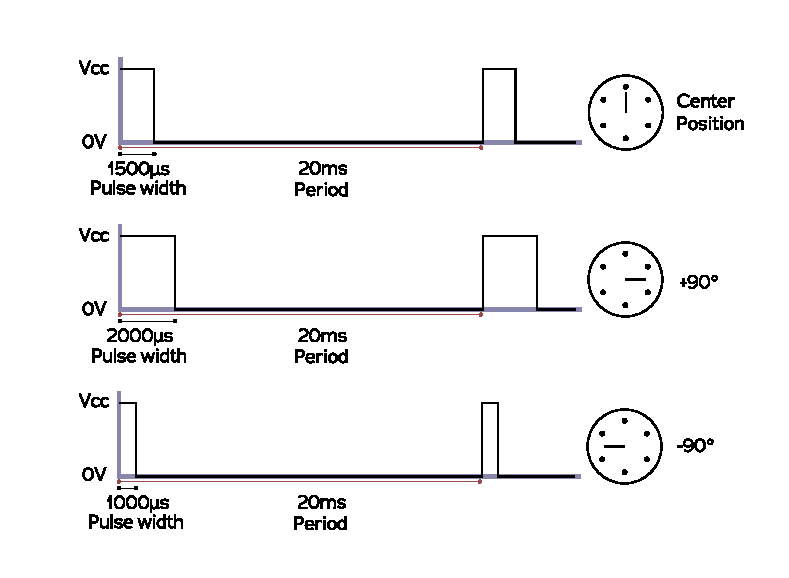
\includegraphics[width=0.7\linewidth]{fig/Servomotor_Timing_Diagram.pdf}
\caption{Servomotor timing diagram \cite{servo_control}}
\label{fig:servo_control}
\end{figure}

The servo used in the car is TowerPro MG995. It has metal gears and operating voltage between \SI{4.8}{\V} to \SI{6.6}{\V}. Speed and torque depend on the supply voltage. According to the product specifications [\todo citace], the servo can achieve operating speed of $0.2\, \text{s}/60^\circ$ and torque of \SI{9.4}{\kg\per\cm} with the \SI{4.8}{\V} supply voltage. From the operating speed we can calculate angular velocity: 
\begin{equation}
\omega = \frac{d \theta}{d t} = \frac{\frac{\pi}{3}}{0.2} \doteq 5.236\ \unit{\radian\per\second}\ .
\end{equation}
Since the servo supply voltage is \SI{5}{\V}, both speed and torque values should be slightly higher.


\section{Motor and ESC}
\label{sec:hw_bldc}
As mentioned in section \ref{sec:hw_mods}, the biggest BLDC with a shaft diameter of \SI{2}{\mm} was selected to replace the old brushed one. The motor was supplied in a set including a \SI{25}{\A} Electronic Speed Controller (ESC). The type is GoolRC 2435 \SI{4800}{\Kv}\footnote{\unit{Kv} refers to rpm/min/V with no load attached to the motor} BLDC; available information about the motor is in table \ref{tab:BLDC_spec} and about ESC in table \ref{tab:ESC_spec}. Since the BLDC motor is directly connected to the ESC and the car communicates only with the ESC, the BLDC is considered a black box.

RC ESCs are controlled the same way as RC servos; thus, the same timing diagram in figure \ref{fig:servo_control} applies. The only difference is the resulting motion. Pulse width with a duration of \SI{2}{\ms} equals full forward acceleration, pulse width with a duration of \SI{1.5}{\ms} equals neutral, and pulse width with a duration of \SI{1}{\ms} equals full brake/reverse.

Whether the brake or reverse is activated depends on the actual motion of the motor. If the car is going forward (meaning the motor rotates forward) and the pulse width becomes lower than \SI{1.5}{\ms}, first, the brake is activated and remains activated until the pulse width is again \SI{1.5}{\ms} or greater. The car must be almost static to start reversing; otherwise, the ESC will stay in brake mode. If the car is static or is already reversing, a pulse width lower than \SI{1.5}{\ms} activates reverse mode.

\begin{table}[t]
   %\renewcommand{\arraystretch}{1.1}
   \tabcolsep 18pt
   \centering
    \caption{BLDC specifications}\label{tab:BLDC_spec}   
    \begin{tabular}{l r}
       \noalign{\hrule height 1.1pt}\noalign{\smallskip}	   
	Power			& 300\unit{\W}\\
	Max. voltage   	& 12.6\unit{\V}\\
	Max. current   	& 24\unit{\A}\\
	Rotor poles	   	& 4 \\
	\unit{\Kv} rating	  	& 4800 \\
	Length			& 24\unit{\mm} \\
	Diameter			& 35\unit{\mm} \\
	Shaft diameter	& 2\unit{\mm} \\
       \noalign{\smallskip}\noalign{\hrule height 1.1pt}
    \end{tabular}
\end{table} 
\begin{table}[t]
   %\renewcommand{\arraystretch}{1.1}
   \tabcolsep 12pt
   \centering
    \caption{ESC specifications}\label{tab:ESC_spec} 
    \begin{tabular}{l r}
       \noalign{\hrule height 1.1pt}\noalign{\smallskip}
	Continuous current		& 25\unit{\A}\\
	Instantaneous current   	& 50\unit{\A}\\
	BEC type				   	& 5\unit{\V}, 2\unit{\A}\\
	Battery				   	& 2-3 Cell LiPo \\
       \noalign{\smallskip}\noalign{\hrule height 1.1pt}
    \end{tabular}
\end{table} 

\section{Control board}
\label{sec:hw_control}
Prototyping was mainly done on the breadboard using the RobotDyn's BlackPill development board featuring STM32F303CCT6 microcontroller \cite{black_pill}. The board uses a similar size and form factor as the popular BluePill board equipped with STM32F103C8T6 \cite{blue_pill}. Both these boards were readily available. BlackPill was selected for its better processor based on an ARM M4 core with FPU, larger memories, and more advanced peripherals. The board is shown in figure \ref{fig:black_pill}.
\begin{figure}[t]
\centering
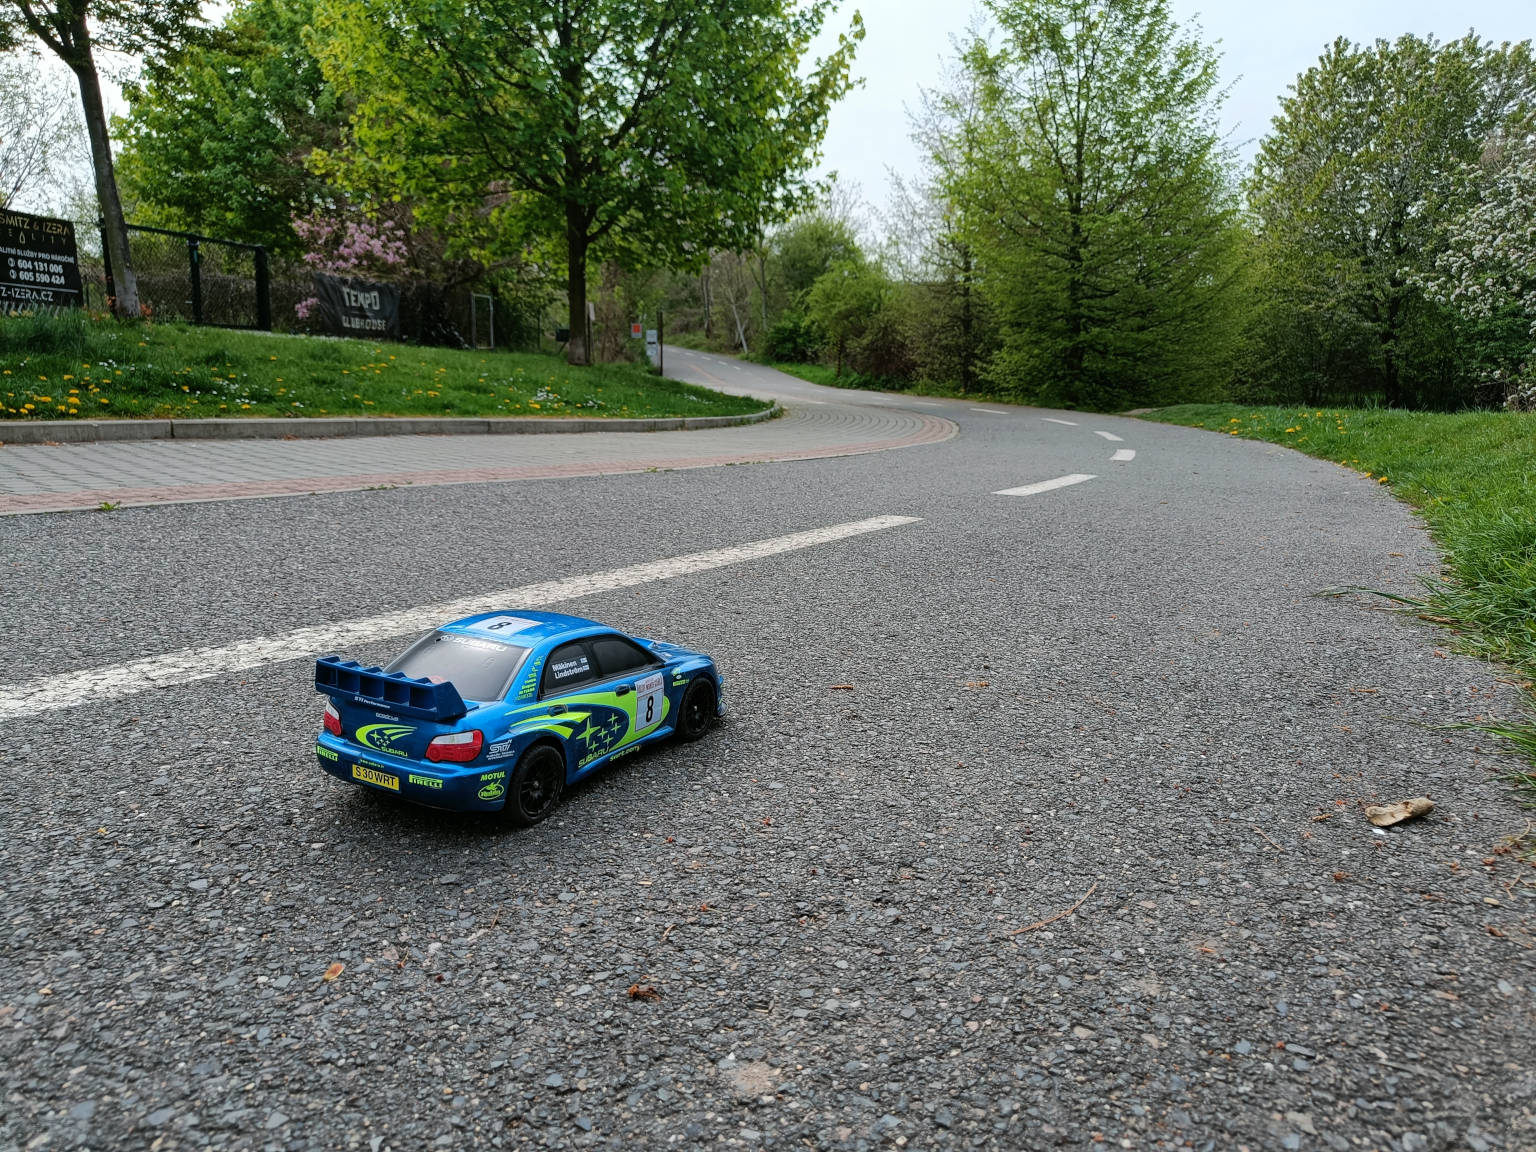
\includegraphics[width=0.5\linewidth]{support/pic/placeholder.jpg}
\caption{*PLACEHOLDER* RobotDyn BlackPill development board}
\label{fig:black_pill}
\end{figure}


\section{Communication}
\label{sec:hw_comm}
The project uses wireless modules equipped with nRF24L01+ transceiver chip from Nordic Semiconductor [\todo citace], a power amplifier, a low-noise amplifier, and an external antenna. The chip operates in the worldwide \SI{2.4}{\GHz} ISM band and communicates with the MCU using the SPI bus. Configurable parameters include channel, data rate, and output power. These modules fit all the requirements, and in addition, they are cheap and readily available.

According to the product specification [\todo cit-Amazon], the range should be more than \SI{800}{\m} line-of-sight. Thanks to the Enhanced ShockBurst protocol and its Auto Acknowledgement function [\todo citace], attaching a small payload to the ACK packet is possible. This feature is advantageously used to report car status back to the transmitter.


\section{Sensors}
\label{hw_sensors}
In addition to measuring the voltage, which is necessary for battery monitoring and is realized using a voltage divider, the car also measures current and BLDC case temperature. It is also equipped with 6-axis IMU. In the project's present state, data from sensors are mainly informative and are not used for control purposes.

The transmitter does not use any particular sensor; only battery voltage is measured.

\subsection{Current}
The current is measured using a module with a 30A version of an ACS712 chip. It is a small linear current sensor based on the Hall effect. Current flowing through the sensor's copper terminals generates a magnetic field, which is then sensed by the integrated Hall-effect circuit. The output of the sensor is a voltage proportional to the flowing current. Current sense terminals are electrically isolated from the rest of the sensor; therefore, it is possible to measure high voltages without external electrical isolation. The sensor is capable of measuring both AC and DC current with a stated total output error of $1.5\%$ [\todo citace]. 

\subsection{Temperature}
A digital thermometer DS18B20 provides temperature measurement. The sensor is manufactured by Dallas Semiconductor, which Maxim Integrated later acquired. It can measure temperatures from \SI{-55}{\degreeCelsius} to \SI{125}{\degreeCelsius}. It has a programmable resolution ranging from 9 to 12 bit and $\pm$\SI{0.5}{\degreeCelsius} over most of the measuring range. The sensor uses a 1-Wire interface, which requires only one pin for communication. When combined with parasitic power mode, the whole thermometer requires only two pins for operation [\todo citace].

The project uses the TO-92 package, which was advantageous because of the limited space around the BLDC. The small size made it possible to mount the sensor on the back of the motor housing with the aid of heat-conducting foil.

\subsection{IMU}


\section{Status info}
\label{hw_status}
Neither the RC car nor the transmitter reported any status in the original version. The user had to check the battery state himself; otherwise, the battery could be discharged entirely and damaged. Since LiPo batteries should not be discharged below a certain threshold, the usual rule of thumb across the RC community is not to discharge the battery below \SI{3.1}{\V} per cell, it was necessary to report the battery status.

An RGB LED was chosen for that purpose because it is possible to quickly report the various states to the user using different colors. On the other hand, it is unsuitable for visualizing values such as temperature. Besides, the transmitter has its own battery, whose status should also be reported to the user, and that would need 2 LEDs. The single RGB LED was therefore insufficient for the transmitter.

For this reason, the display seemed like a good alternative and replacement. An OLED display was convenient as its power consumption is low, it is readable in direct sunlight, and thanks to only one color, it is fast. The disadvantage is its small size, which complicates the orientation in the displayed data.

Considering all the factors, both the RGB LED and the OLED display were used. RGB LED serves as a fast state notifier, and further status information can be found on the display.

Both car and transmitter use RGB LED with a common anode and monochrome OLED display module with SSD1306 chip communicating using I\textsuperscript{2}C bus [\todo citace].


%\begin{table}[t]
%\centering
%\caption{*PLACEHOLDER* BLDC specifications} %TODO citace
%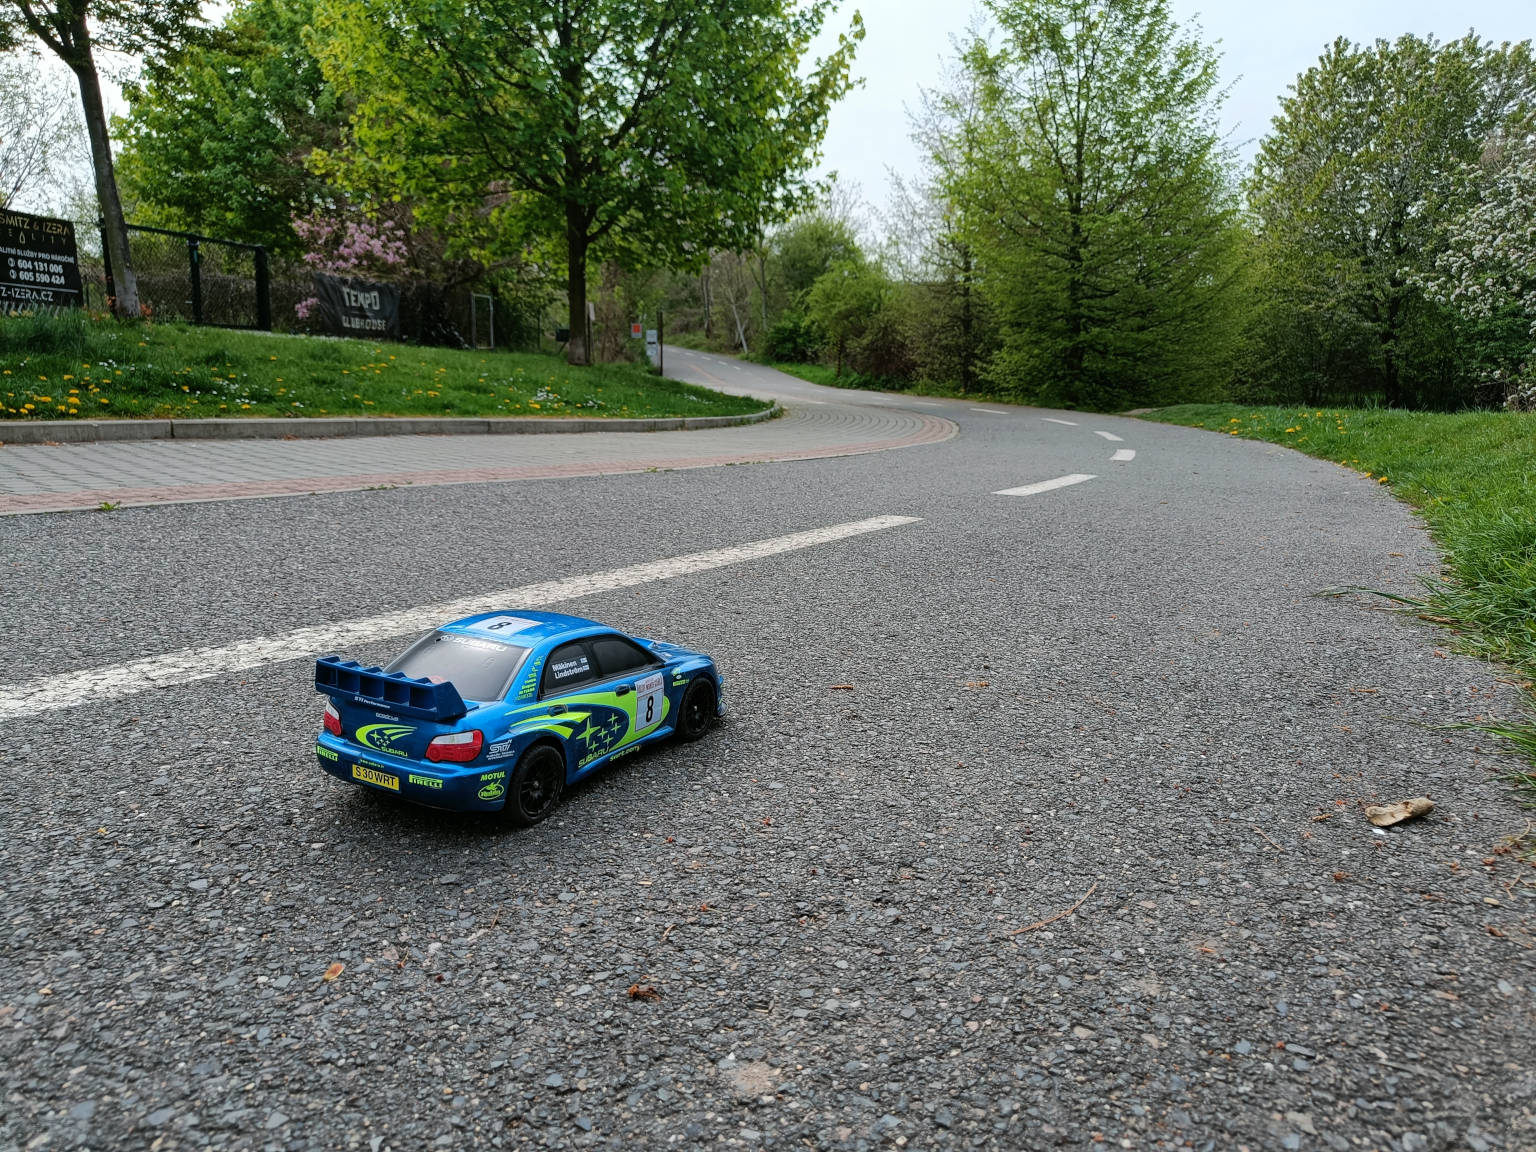
\includegraphics[width=0.8\linewidth]{support/pic/placeholder.jpg}
%\label{tab:BLDC_spec}
%\end{table}


	\clearpage
	
%!TEX ROOT=main.tex


\part{Realization}
\label{chap:realization}
Since there are no spare parts available for the transmitter or the car, all modifications have been made with as little structural intervention as possible. This process can be referred to as retrofitting.

\section{Transmitter}
\label{sec:real_tx}
\subsection{Power supply}
As described in section \ref{sec:hw_mods}, the transmitter is powered by a 2-cell LiPo battery with a nominal voltage of \SI{7.4}{\V}. The battery is connected via an XT60 connector and a switch to a step-down converter module with an LM2596 chip. The module is needed to regulate the battery voltage to \SI{5}{\V} to power the control board.

This voltage is used for the RGB LED, communication module, and linear voltage regulator AP2111, which regulates it to \SI{3.3}{\V} used to power the rest of the components. This regulator was selected because of the low dropout voltage of only \SI{250}{\mV} and high output current of \SI{600}{\mA} \cite{ap_datasheet}.		%TODO measure TX current?

In order to measure the battery voltage with the processor's internal ADC, it first had to be lowered to fit within the ADC range, which is $0\, \text{-}\, 3.3$\unit{\V}. Therefore a voltage divider is soldered to the input terminals of the step-down module. The divider was designed to use resistors with standard values and is pictured in figure \ref{fig:tx_div}. The resistor values are R1 = \SI{22}{\kohm}, R2 = \SI{10}{\kohm}.
\begin{figure}[ht]
\centering
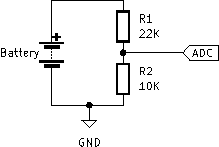
\includegraphics[width=0.4\linewidth]{fig/voltage_divider.pdf}
\caption{Voltage divider utilized in the transmitter }
\label{fig:tx_div}
\end{figure}

A fully charged 2-cell LiPo battery reaches \SI{8.4}{\V}, then the output of the divider equals
\begin{equation}
	U_{adc} = U_{batt} \cdot \frac{R2}{R1+R2} = \SI{2.625}{\V}\ ,
\end{equation}
which is safely within the ADC range.

\subsection{Controls}
The transmitter was supplied with a steering wheel and trigger as 5kohm potentiometers. Since they are old, a \SI{100}{\nF} capacitor was added between the output pin of both potentiometers and ground to form a low-pass filter and smooth out the output signal.

Potentiometers used for control trimming were replaced with quadrature rotary encoders with push buttons. Encoders have screw threads, as can be seen in figure *fig*, which fit into the original holes. Since encoders are fixed to the transmitter, a simple connector made from a pin socket was soldered to encoder pins [TODO: fotka].

\subsection{PCB design}
	\clearpage
	
%!TEX ROOT=main.tex


\part{Software}
\label{chap:software}
\section{Introduction}
The control program for both the transmitter and the car is written in C language. It utilizes the STM32 HAL (Hardware Abstraction Layer) libraries, and the STM32CubeMX graphical utility was used to set up the necessary initialization and project files and generate code for peripheral configuration. Afterward, the application is compiled using a Makefile under Linux by the GNU GCC cross-compiler for ARM bare-metal targets.

STM32 HAL driver library provides a set of APIs to simplify interaction with all the peripherals and thus the user application implementation. The HAL driver layer implements run-time failure detection to increase robustness. HAL APIs are available for all peripherals. Also, the API ensures high portability across different STM32 families \cite{hal}.

STM32CubeMX is a graphical tool that provides a convenient user interface to configure the microcontroller. It allows a simple configuration of pin assignments, peripherals, or the clock tree, and the corresponding C initialization code generation. It also packs middleware stacks, such as USB, FatFs, or TCP/IP. This tool notably speeds up the process of microcontroller configuration and allows the user to focus on the application \cite{cubemx}.

The control program is almost exclusively interrupt-driven. Emphasis has been placed on program execution speed to ensure a high frequency of control commands and, therefore, smooth car control.

\section{File structure}
Software for both the transmitter and car is in their respective folders. STM32CubeMX generated the code, and to maintain compatibility, the dedicated user code sections were used. The code was generated with CubeMX's basic application structure setting.

Therefore both project folders in the \textit{'Software'} folder contain the \textit{'Drivers'} folder with ARM and HAL drivers for the board, the \textit{'Inc'} folder with header files, and the \textit{'Src'} folder with source files. The startup file, makefile, linker script, and CubeMX project file are in the root folder. As the car implements FatFs driver, it is located mainly in the \textit{'Middlewares'} folder.

The \textit{'shared\_libs'} folder contains shared libraries for both applications, namely the nRF24 module and OLED display libraries, and follows the same file structure; the \textit{'Inc'} folder contains header files and the \textit{'Src'} folder source files. Icons used on the OLED display are in the dedicated \textit{'logos'} folder inside the \textit{'Inc'} folder.

In addition, there are three important files:
\begin{itemize}
	\item \begin{description}
\item[\textit{'project\_tamiya.h'}:]
Shared header located in the \textit{'shared\_libs/Inc'} folder. It contains common libraries and \textit{'platform.h'} file. More importantly, it contains nRF24 communication settings, various macros, and shared function declarations, namely nRF24 and OLED wrapper functions and functions used for UART debug prints.
\end{description}

	\item \begin{description}
\item[\textit{'project\_tamiya.c'}:]
Source file located in the \textit{'shared\_libs/Src'} folder. It consists of function definitions from the appropriate header file.
\end{description}

	\item \begin{description}
\item[\textit{'platform.h'}:]
This header file is in both applications' \textit{'Inc'} folder, contains platform-specific macros and settings, and includes platform-specific headers.
\end{description}
\end{itemize}
The visualization of the file structure with highlighted important files is below.

\begin{forest}
  pic dir tree,
  pic root,
  for tree={% folder icons by default; override using file for file icons
    directory,
  },
  [Software
    [Car, label=right:Main folder of the car control application
    		[Inc
    			[platform.h, file
    			]
    		]
    ]
    [shared\_libs, label=right:Shared libraries for both applications
    		[Inc
    			[project\_tamiya.h, file
    			]
    		]
    		[Src
    			[project\_tamiya.c, file
    			]
    		]
    ]
    [Transmitter, label=right:Main folder of the transmitter control application
    		[Inc
    			[platform.h, file
    			]
    		]
    ]
  ]
\end{forest}

\subsection{Communication parameters}
Since the communication parameters must be equal in both the car and transmitter to establish the connection, they are placed in the shared \textit{'project\_tamiya.h'} header file.

The control packet payload size is only 4 bytes, and the ACK packet payload is only 3 bytes. In addition, 1 byte CRC is used. Payloads are described in figures \ref{tab:ctrl_payload} and \ref{tab:ack_payload}. CRC and other fields of the \textit{Enhanced ShockBurst} packet are not displayed.

\begin{figure}[ht]
\centering
	\begin{bytefield}[bitwidth=1.2em, bitheight=2em]{32}
        \bitheader{0, 8, 16, 24, 32} \\
        \bitbox{16}{Throttle} & \bitbox{16}{Steering}
    \end{bytefield}
    \caption{Control payload format}
    \label{tab:ctrl_payload}
\end{figure}
	
\begin{figure}[ht]
\centering
	\begin{bytefield}[bitwidth=1.5em, bitheight=\widthof{~\small$\frac{1}{2}$\unit{\celsius}~}]{24}
        \bitheader{0, 8, 16, 17, 24} \\
        \begin{rightwordgroup}{RTP \\  Header}
        \bitbox{16}{Battery voltage} & \bitbox{1}{\rotatebox{90}{\small$\frac{1}{2}$\unit{\celsius}}} & \bitbox{7}{Integer temperature}
    \end{bytefield}
    \caption{ACK payload format}
    \label{tab:ack_payload}
\end{figure}
\noindent
Bit 16 of the ACK payload is related to the trick described in \ref{sub:integers}.

The channel frequency is set to \SI{2515}{\MHz} to reduce interferences with the wi-fi signal, and the data rate is the lowest possible \SI{250}{\kilo\bit\per\second}. According to \cite{nrf_datasheet}, a lower air data rate gives better receiver sensitivity than a higher air data rate. Transmitting power is, on the other hand, the highest possible. This setup ensures the most extended potential range.


\section{Transmitter}
\subsection{Peripherals and pin configuration}
\label{sub:tx_conf}
\begin{figure}[h]
\centering
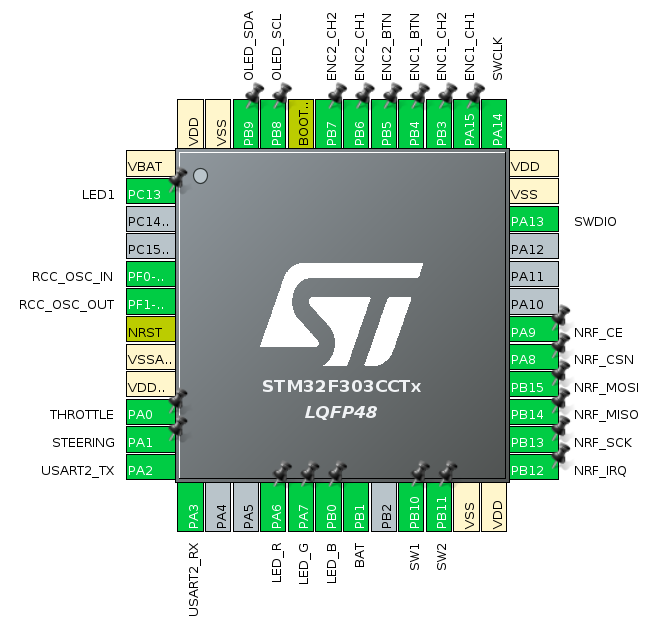
\includegraphics[width=0.7\linewidth]{fig/tx_pin_assignments.png}
\caption{Transmitter pin assignments}
\label{fig:tx_conf}
\end{figure}
\noindent
The microcontroller runs at \SI{72}{\MHz} with a clock source set to a \SI{12}{\MHz} external crystal oscillator.

ADC1 channels 1 and 2 are used to measure the output voltage from control potentiometers. ADC operates with 12-bit resolution in continuous conversion mode with DMA enabled in circular mode with continuous requests to manipulate the data. Once the ADC conversion is started, it remains active, and DMA repeatedly fills the buffer with measured data. Sampling time is the highest possible 601.5 cycles, and software averaging is used to acquire stable measurements.

ADC3 uses channel 1 to measure the LiPo battery voltage and channel Vrefint to measure the internal reference voltage. Again, the resolution is 12-bit, continuous conversion mode is enabled, and DMA is utilized to transfer data from peripheral to memory. In this mode, the ADC remains active until DMA fills the whole data buffer. The sampling time for channel 1 is $601.5$ cycles, and for channel Vrefint $181.5$ cycles.

The communication module is connected to the SPI2 bus operating in full-duplex master mode. Baud rate is set to \SI{9}{\mega\bit\per\second}, and the data size is standard 8 bits. 'NRF\_IRQ' pin is configured in external interrupt mode with rising edge detection. The rest of the 'NRF' pins are simple outputs.

Quadrature rotary encoders utilize timers TIM2 and TIM4, which are in Encoder mode. This mode is designed specially to interface quadrature encoders with out-of-phase output signals. Encoder push-button pins are configured in external interrupt mode with rising edge detection.

SW1 and SW2 pins belong to the DIP switch and are configured in external interrupt mode with both rising and falling edge detection.

USART2 peripheral is configured as debug serial port. Baud rate is set to \SI{921600}{\bit\per\second} with 8~bits word length and one stop bit.

I2C1 in Fast Mode Plus with a frequency of \SI{1}{\MHz} connects the OLED display. LED pins are simple outputs. Furthermore, TIM6 at \SI{1}{\Hz} and TIM16 at \SI{4}{\Hz}, both timers with interrupts enabled, are used for basic timing purposes.

Figure \ref{fig:tx_conf} shows the complete pinout in STM32CubeMX.

\subsection{Application start}
The program starts with auto-generated initialization of all necessary peripherals. Debug UART is enabled after start by default. Afterward, an orange LED visible from the backside of the transmitter is turned on to indicate application initialization.

First, the OLED display is initialized, and the project logo is displayed. At the same time, a greeting is sent via UART, and the RGB LED flashes through each channel. Automatic self-calibration of both ADCs follows, and the Vrefint calibration value is obtained from the appropriate register. This value is later used to calculate VDDA. Then the communication module is initialized in transmitter mode with parameters defined in \textit{project\_tamiya.h}.

After that, the ADC responsible for reading values of control potentiometers is started in circular DMA mode, as described in section \ref{sub:tx_conf}. Processing of the data is explained in section \ref{sub:adc}.

In the final part of initialization, all the timers, including the timers used for quadrature encoders, are started in interrupt mode. Then the UART is deinitialized depending on the Switch1 state, the orange LED is turned off to indicate that initialization is done, and the program enters the main control loop.

\subsection{Main control loop}
The control loop is designed to be as non-blocking and interrupt-driven as possible. Therefore, it consists of a set of 'if' blocks. However, some parts remained blocking. The reason is some of the drivers are blocking and do not allow the use of DMA. Rewriting them was hardly possible or too time-consuming. This is especially true for OLED refreshing, which takes the longest time. Execution of given 'if' block is controlled by flags, internally boolean values, set by appropriate interrupt routines.
\begin{itemize}
	\item \begin{description}
\item[\textit{'trigger\_data\_rdy'}:]
The flag is set by ADC interrupt routines and indicates available control values. This block processes and averages measured values from control potentiometers and recalculates them using hardware limits for direct usage in the car. The flag is reset at the end of the block.
\end{description}

	\item \begin{description}
\item[\textit{'adc\_data\_bat\_rdy'}:]
This block is similar to the previous block and indicates available voltage measurements.  First, it averages the measured Vrefint and battery voltage data. The next step is VDDA calculation:
\begin{equation}
	V_{DDA} = \frac{\SI{3.3}{\V} \cdot Vrefint_{cal}}{Vrefint_{meas}}\ ,
\end{equation}
where $Vrefint_{cal}$ is a value acquired during the manufacturing process at $V_{DDA} = \SI{3.3}{\V}$ and obtained from the register, and $Vrefint_{meas}$ is measured internal reference voltage. The formula was taken from Section 15.3.32 in \cite{f303_ref}. This computed value is used to convert the ADC battery measurement to the actual voltage.

The corresponding ADC sets the flag, and the program resets it at the end of the block. A~\SI{4}{\Hz} timer triggers the ADC measurement itself.
\end{description}

	\item \begin{description}
\item[\textit{'sending'}:]
This is the first phase of the non-blocking packet transmission routine. It is executed only if the flag is false, indicating that the previous transmission is completed. First, the flag is set, trimming values are added to the control values from potentiometers, and a 4-byte data packet is formed. After that, packet transmission is started. The flag remains set.
\end{description}

	\item \begin{description}
\item[\textit{'NRF\_IRQ'}:]
This is the second, final phase of the packet transmission routine. The communication module's interrupt pin sets the flag once it finishes the transmission. The routine starts with checking the transmission status and reading the received payload. If the payload has the expected size, it is parsed into related variables. Then actions depending on the transmission status follow.

The corresponding counter variable is incremented if the module has reached the maximum retransmit count. This variable is used to detect signal loss as described in section \ref{sub:tx_sig_loss}. If the transmission was successful, the previously mentioned variable is reset, the command frequency counter is incremented, and the status LED is toggled.

The last step is resetting both the \textit{'NRF\_IRQ'} and \textit{'sending'} flags.
\end{description}

	\item \begin{description}
\item[\textit{'display\_refresh'}:]
This section is responsible for refreshing the information on the OLED display. An interrupt routine of a \SI{4}{\Hz} timer sets the flag, and the program resets it at the end of the block. Therefore, the display runs with a framerate of about \SI{4}{FPS}.
\end{description}

	\item \begin{description}
\item[\textit{'ENCx\_IRQ'}:]
This section is executed when the rotary encoder's control timer triggers the interrupt routine upon detecting rotation. Depending on the direction of rotation, the trimming value is increased or decreased. The flag is reset at the end of the block.

Each encoder has its own control block modifying the appropriate trimming value.
\end{description}

	\item \begin{description}
\item[\textit{'ENCx\_reset'}:]
This flag is set by the encoder's push-button. The purpose is to reset the appropriate trimming value to zero. At the end of the block, the flag is reset.
\end{description}

\end{itemize}


\subsection{ADC data processing}
\label{sub:adc}
A feature similar to 'double buffering' is implemented to process data from ADC in circular mode. It is not implemented as two separate buffers but as a single 1024 bytes long buffer. It utilizes the ADC ability to send notifications when the buffer is half-full and when it is full.

ADC is enabled and DMA starts filling the buffer with data. Once the buffer is half-full, the appropriate interrupt is triggered, and MCU is signaled to start processing the first half of the buffer. The DMA still fills the buffer with new data.

When the DMA fills the buffer completely, the appropriate interrupt is triggered, and the DMA starts filling the buffer from the beginning with new measurements. This state is again signaled to the MCU, which starts processing the second half of the buffer while the DMA fills the first half.

Whether the first or the second half is to be processed is controlled by an integer offset that is set in the interrupt routine. Hence, this method is fast as the DMA still fills the same buffer and does not need to be reconfigured, which would add additional overhead.

This approach is repeated, ensuring that the new measurements do not overwrite the values already in the buffer and, therefore, do not affect the value obtained.

\subsection{Signal quality and loss detection}
\label{sub:tx_sig_loss}
The nRF24 communication module does not support any detailed form of RSSI (Received Signal Strength Indicator). The only information obtainable from the module is whether the signal during the last transmission was below or under a certain threshold. Therefore, a simple signal quality indicator is implemented in the software.

After every successful packet transmission, the counter variable \textit{'tx\_freq\_cnt'} is incremented. During the callback routine of a 1Hz timer, this value is copied into \textit{'tx\_freq'} variable and displayed. This value, expressing the number of packets per second, is used to measure the signal quality. Thresholds were determined experimentally based on the maximum observed number of packets per second.

Since the detection of signal loss by the transmitter is not as important as in the case of a car and serves mainly for information purposes, the implementation is quite simple.

It depends on the counter variable \textit{'retransmits\_in\_row'}, which is incremented whenever the communication module reaches the maximum number of packet retransmits and reset if the transmission was successful. When this variable is greater than 15, it is evaluated as a signal loss in the 4Hz timer interrupt routine, and the corresponding flag is set.

This status is visualized on the OLED screen and by changing the color of the status LED to blue.

\subsection{Status visualization}
Both the RGB LED and OLED display are used to visualize the current status. The reasons for the choice are discussed in section \ref{sec:hw_status}.

The RGB LED is clearly visible and serves as a quick notification of the communication and the transmitter's battery status. Color options and their meaning are described in table \ref{tab:led_status}.
\begin{table}[ht]
   \renewcommand{\arraystretch}{1.1}
   \centering
    \caption{Explanation of LED status}\label{tab:led_status}   
    \begin{tabular}{c c c}
       \noalign{\hrule height 1.1pt}\noalign{\smallskip}
	   \bfseries RGB LED & \bfseries Communication status & \bfseries Battery status\\[0.2em]
	\noalign{\hrule height 1.1pt}\noalign{\smallskip}     
flashing green	& OK				& $>\,$\SI{6.8}{\V} \\
flashing red		& OK				& $<\,$\SI{6.8}{\V} \\
blue				& signal lost	& --	\\
       \noalign{\smallskip}\noalign{\hrule height 1.1pt}
    \end{tabular}
\end{table} 

The small OLED display is more demanding for quick orientation in the displayed data. On the other hand, it provides more information about the transmitter and even the car. The display interface is divided into two main parts.

The first in the upper part of the display resembles a status bar and provides information about the car, as indicated by the icons: the BLDC temperature and battery state. In case of signal loss, this information is displayed here.

The rest of the screen is separated by a line and belongs to the transmitter status. Information about the current position of control potentiometers is displayed in the middle, along with the trim values. The position of potentiometers is not expressed relatively in percentage. Instead, the actual value sent to the car is displayed. The bottom part offers information about packets per second and the transmitter's battery status.

Both battery indicators are interactive and, depending on the voltage, up to 4 bars are displayed. If the battery voltage drops below the threshold of \SI{6.8}{\V}, a flashing exclamation mark is displayed in the battery logo instead. The signal quality indicator is also interactive.

All logos were created in GIMP and exported as XBM files. These were later 'converted' to header files by changing the file extension. Examples of the display interface are in figure \ref{fig:tx_oled}.
\begin{figure}[t]
    \centering
    \begin{subfigure}{0.35\textwidth}
    \centering
        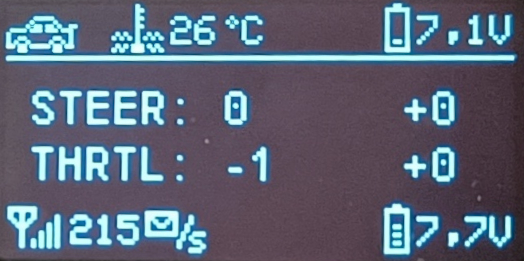
\includegraphics[width=1\textwidth]{fig/tx_oled_ok.jpg}
%		\caption{front side}
    \end{subfigure}%
    \hspace{1cm}
    \begin{subfigure}{0.35\textwidth}
    \centering
		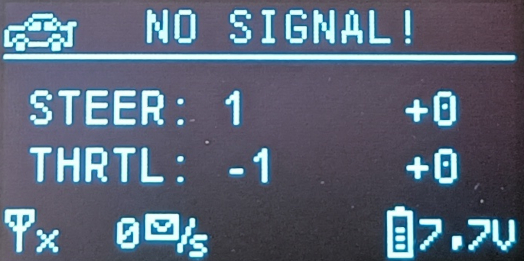
\includegraphics[width=1\textwidth]{fig/tx_oled_nosig.jpg}
%		\caption{back side}
    \end{subfigure}
	\caption{OLED display interface in transmitter}
    \label{fig:tx_oled}
\end{figure}

\subsection{UART debug prints}
One of the UARTs is utilized for printing debug information. Corresponding pins are available on the connector J3; configuration is in section \ref{sub:tx_conf}.

The printing is enabled by default after the application start and prints the initialization progress. Afterward, the printing is dependent on the state of the Switch1 (the first lever on the DIP switch SW2).

The UART is deinitialized before entering the main control loop if the switch is in the off position or stays initialized otherwise. If debug prints are enabled, the transmitter informs about:
\begin{itemize}
\item LiPo battery voltage and VDDA voltage whenever new data is available,
\item encoder rotation,
\item switch position change,
\item no signal state.
\end{itemize}
Debug printing can be enabled or disabled anytime during the application execution.



\section{Car}
\subsection{Peripherals and pin configuration}
\label{sub:car_conf}
\begin{figure}[h]
\centering
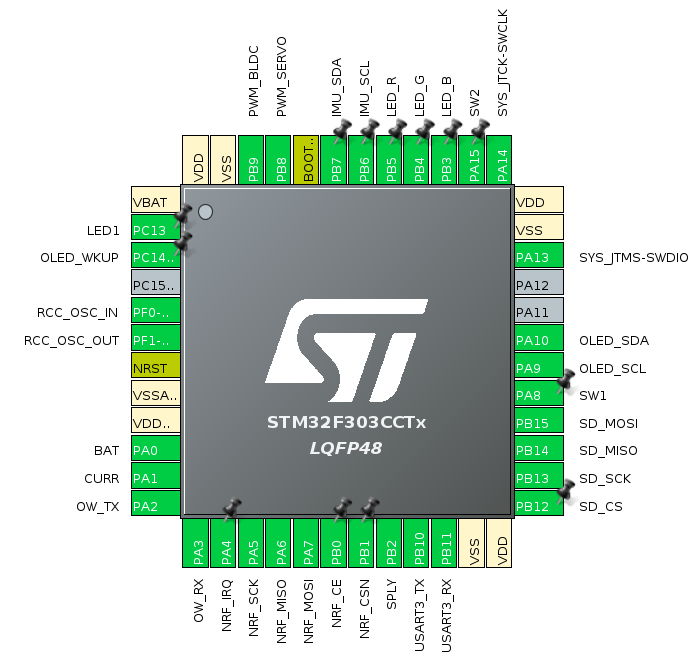
\includegraphics[width=0.75\linewidth]{fig/car_pin_assignments.png}
\caption{Car pin assignments}
\label{fig:car_conf}
\end{figure}
Some of the settings are similar to transmitter settings since both microcontrollers are the same STM32F303CCT6. The microcontroller runs at \SI{72}{\MHz} with a clock source set to an \SI{8}{\MHz} external crystal oscillator.

Channels 2 and 3 of timer TIM8 are used to generate PWM and therefore control the car. Prescaler and counter period values are calculated to represent the pulse width in microseconds. That means the counter value of e.g. $1500$ equals \SI{1500}{\micro\second} pulse width, which is convenient for control application implementation.

ADC1 channels 1 and 2 are used to measure the LiPo battery voltage and output voltage from the current sensor. ADC operates with 12-bit resolution in continuous conversion mode with DMA enabled. Sampling time is again the highest possible $601.5$ cycles to acquire stable measurements.

ADC2 measures the Vrefint channel to obtain the internal reference voltage and channel 12 to obtain the BEC output voltage. The resolution is also 12-bit, and continuous conversion mode with DMA is enabled. The sampling time for channel Vrefint is $181.5$ cycles and $601.5$ cycles for channel~12.

The communication module is connected to the SPI1 bus operating in full-duplex master mode. Baud rate is set to \SI{9}{\mega\bit\per\second}, and the data size is standard 8 bits. 'NRF\_IRQ' pin is configured in external interrupt mode with rising edge detection. The rest of the 'NRF' pins are simple outputs.

As STM32F303 does not support the SDIO interface, the SD card is connected via the SPI2 peripheral. The baud rate is only \SI{281.25}{\kilo\bit\per\second} after reset, but once the SD card is initialized, it is increased to \SI{9}{\mega\bit\per\second}.

I2C2 in Fast Mode Plus with a frequency of \SI{1}{\MHz} connects the OLED display. IMU unit is served by I2C1 in Fast Mode with a frequency of \SI{400}{\kHz}.

1-Wire bus necessary to communicate with the DS18B20 temperature sensor is implemented using USART2 peripheral and DMA. This method is described in \cite{1wire_uart}, and the DMA version was implemented with the help of \cite{1wire_uart_imp}. Since RX and TX pins are tied together, and TX pin is configured as push-pull, it is protected with a diode. This method is much simpler and requires fewer external components than the approach in \cite{1wire_uart} with a discrete open-drain buffer.

SW1 and SW2 pins belong to the DIP switch and are configured in external interrupt mode with both rising and falling edge detection.

USART3 peripheral is configured as debug serial port. Baud rate is set to \SI{921600}{\bit\per\second} with 8~bits word length and one stop bit.

LED pins are simple outputs. Pins PA11 and PA12 are not used in the project's current state but are reserved for a USB peripheral for possible future expansion with a control computer.

Figure \ref{fig:car_conf} shows the complete pinout in STM32CubeMX.

\subsection{Application start}
The application for controlling the car is written similarly to the transmitter. The program starts with the initialization of all peripherals. Debug UART is enabled after start by default, too, and a blue LED on the BlackPill board indicates application initialization.

First, the OLED display is initialized, and the project logo is displayed. At the same time and a greeting is sent via UART. If the Switch2 is turned on, IMU is initialized, and the flag controlling SD card logging is set. The next step is enabling servo and motor PWMs, initializing 1-Wire, and flashing individual channels of RGB LED.

Automatic self-calibration of both ADCs follows, and the Vrefint calibration value is obtained from the appropriate register. This value is later used to calculate VDDA. Then the communication module is initialized in receiver mode with parameters defined in \textit{project\_tamiya.h}.

After that, depending on the Switch2 position, the SD card is initialized and mounted. This process is explained in more detail in section \ref{sub:sd_log}.

Lastly, all the timers are started in interrupt mode. Timer TIM15 controlling the display timeout is immediately stopped afterward. This is because the timer triggers an interrupt when started for the first time even though it is not supposed to, which interferes with the display timeout feature.

Then the OLED display is turned off, UART is deinitialized depending on the Switch1 state, and the blue LED is turned off to indicate that initialization is done. The run time in milliseconds is stored just before entering the main control loop for possible later calculation of the data timestamp.

\subsection{Main control loop}
The following section describes the control loop. Similar to the transmitter control loop, it is designed to be as non-blocking and interrupt-driven as possible and consists of a set of 'if' blocks accordingly. The biggest bottleneck is the FatFs driver used for SD card logging, which is too complex to rewrite in DMA mode and takes the longest execution time. Individual 'if' blocks are controlled by their appropriate flag.

\begin{itemize}
	\item \begin{description}
\item[\textit{'NRF\_IRQ'}:]
The flag is set by the communication module and indicates the module's status change. If the status represents newly received data, an ACK packet is first prepared and sent back to the transmitter to confirm successful reception. If the received data has the expected size, processing follows.

Received values are checked against the defined chassis mechanical limits and clipped if they exceed the allowed range. After that, values are recalculated to pulse widths and set into PWM generating timers. Lastly, the safety timer is reset, and the command frequency counter is incremented. The flag is reset by the program at the end of the block.
\end{description}

	\item \begin{description}
\item[\textit{'temp\_conv\_ready'}:]
Although it may seem like the temperature sensor controls this flag, it is actually controlled by a \SI{1}{\Hz} timer. The temperature sensor datasheet states that temperature conversion with 12-bit resolution takes \SI{750}{\ms} and, therefore, one-second intervals are sufficient.

Nevertheless, this section indicates that the temperature conversion is done, and the reading process can be started. If SD logging is enabled, it also flushes cached data to the SD card with the \textit{'f\_sync'} function.
\end{description}

	\item \begin{description}
\item[\textit{'temp\_received'}:]
This is the section controlled by the temperature sensor. The flag is set by a~\mbox{1-Wire} interrupt and indicates that the measured data transfer from the sensor has finished. Thus the raw register data is converted to the actual temperature. The process is mentioned in section \ref{sub:integers}.

Lastly, the flag is reset, and the following temperature conversion is initialized.
\end{description}

	\item \begin{description}
\item[\textit{'adc\_data\_bat\_rdy'} and \textit{'adc\_data\_sply\_rdy'}:]
Appropriate ADC callback routines set flags. Both of them must be set to execute this block, which is responsible for processing data. First, measurements from both ADCs are averaged to obtain stable values. The VDDA calculation and conversion of values to the relevant physical quantities follows. Then if SD logging is enabled, data from IMU is read, and all the values are formatted and written to the SD card.

At the end of the block, both flags are reset. A \SI{50}{\Hz} timer triggers ADCs themselves.
\end{description}

	\item \begin{description}
\item[\textit{'log\_data'} and \textit{'unmount\_sd'}:]
This block ensures safe unmount and disconnection of the SD card. The file is truncated, closed, and the SD card is unmounted. If Switch2 is turned on after the start of the application, the \textit{'log\_data'} flag is set. The \textit{'unmount\_sd'} flag is set if it is turned off during execution. Both flags are reset at the end of the block.
\end{description}

	\item \begin{description}
\item[\textit{'display\_refresh'} and \textit{'display\_wakeup'}:]
This section is responsible for refreshing the information on the OLED display if it is turned on. An interrupt routine of a \SI{4}{\Hz} timer sets the \textit{'display\_refresh'} flag, and the program resets it at the end of the block. The \textit{'display\_wakeup'} flag is set for 5 seconds by pressing the push-button under the display, which also activates it.
\end{description}

\end{itemize}


\subsection{Integer arithmetics}
\label{sub:integers}
Although the selected MCU contains the FPU, all program variables are integers. The problem is not the speed of floating-point operations. Floating-point operations are fast thanks to the FPU and are used in some parts of the program, mainly during converting ADC value to actual voltage.

The problem is that formatting floats for output is slow and, in addition, requires a special flag for the linker and increases the final file size considerably. Hence, float variables are multiplied by~1000 to maintain at least some accuracy and saved as an integer. This approach applies mainly to the accelerometer data. The battery voltage value is already calculated in millivolts to avoid float variables altogether.

An easy 'trick' is utilized to display the BLDC temperature as a decimal number without float variables. The raw register data is converted to the integer part of the temperature using bits 11 to 4, according to Figure 4 in \cite{ds_datasheet}. Then the program checks the value of bit 3 associated with $2^{-1} = \frac{1}{2}$\unit{\celsius} and sets another integer variable to 5 or 0 accordingly. Afterward, the temperature is displayed as two integers with a point between them.

\subsection{Signal quality and loss detection}
\label{sub:safety}
It is expected from an RC vehicle that it safely stops or at least stops the motor in case of signal loss to prevent damage or injury. Since pulse width values controlling the servo and motor are only updated when a new control packet is received, loss of the signal would mean that the last command remains set in PWM generating timer and the car uncontrollably drives away.

One of the timers is used as a 'safety timer' to solve this behavior. The timer is set to \SI{4}{\Hz} with interrupts enabled, and its counter is reset whenever a command packet is successfully received. If no new command is received within \SI{250}{\ms}, the timer triggers an interrupt, resetting the motor and servo to their 'neutral' position and setting the \textit{'no\_signal'} flag. 

Moreover, the associated interrupt callback routine is the only one that directly interferes with car control, which ensures the motor is always reset after exactly \SI{250}{\ms} independently of the current program state if no new command is received.

Theoretically, one of the watchdogs could have been used instead of the timer as a more robust safety measure. However, not reloading it in time would mean restarting the MCU and interfering with SD card data logging.

The signal quality indicator is implemented identically to the transmitter. Each time the packet is successfully received, a counter variable is incremented. The value of the counter variable is copied to another variable and reset every second by a \SI{1}{\Hz} timer. This value is used to estimate signal quality, which is then visualized on the OLED display.

\subsection{SD logging}
\label{sub:sd_log}
A micro SD card slot is ready to use to record driving data. The application implements ChaN's FatFs driver to interface the SD card, and therefore, any FAT-formatted micro SD card can be used. Driving data are saved with a frequency of \SI{50}{\Hz} in CSV file format.

The logged data includes a timestamp, voltage and current measurements, BLDC temperature, actuator control values, and IMU data. The exact format and corresponding units of quantities are always specified in the first two lines of the CSV file.

Data logging is enabled if Switch2 is turned on during the application start. Unlike UART prints, it cannot be enabled anytime. Depending on the Switch2 position, the SD card mounting and preparation procedure is performed right after communication module initialization.

It starts with mounting the disk and printing SD card statistics. Then the application search for the 'logs' folder, and if it is not found, it creates one. Afterward, the files in the folder are counted to determine the log number, and a new file is created.

Then pre-allocation of \SI{10}{\mebi\byte} of memory follows, which should suffice for approximately an \mbox{hour-long} log file. This step is critical as it dramatically decreases filesystem overhead when writing to the file. Without the pre-allocation, the \textit{'f\_sync'} function sometime took so long that the safety timer triggered and reset the motor.

Every second, the log file is \textit{'f\_synced'} to lower its execution time and prevent data loss if an unexpected event happens, such as a shutdown. With this approach, the user should not lose more than the last second of data.

Even though the pre-allocation reduced \textit{'f\_sync'} execution time significantly, it still sometimes takes more than \SI{100}{\ms}, meaning that some data are missing from the log.

Switch2 must be turned off to finish data logging properly. After that, the file is truncated and closed, and the whole SD card is safely unmounted.

\subsection{Status visualization}
Visualization of the status is consistent with the transmitter and utilizes the RGB LED and a bit smaller OLED display. Again, the RGB LED serves as a quick notification of the communication and the car's battery status. In the case of body shell mounting, it is also visible through it and is the only status indicator. The color scheme is the same as in the transmitter, and thus, the same table \ref{tab:led_status} applies.

Since the car is usually driven with a body shell mounted, the display is not visible to the user as it is under the body on the control board. For this reason, the display is turned off the majority of the time. It is activated only during the start of the application to display the project logo. The display can be turned on anytime by pressing the push-button under the display, waking it up for 5 seconds.

The display interface is much more plain than the one in the transmitter. 
Due to the size of the display, the only information presented is the battery voltage, motor temperature, and signal quality indicator with packets per second. Both battery and signal indicators are interactive again.

The signal loss is visualized only by the RGB LED and the zero frequency of the commands on the OLED display; no dedicated error message is shown. Examples of the display interface are in figure \ref{fig:car_oled}.
\begin{figure}[t]
    \centering
    \begin{subfigure}{0.4\textwidth}
    \centering
        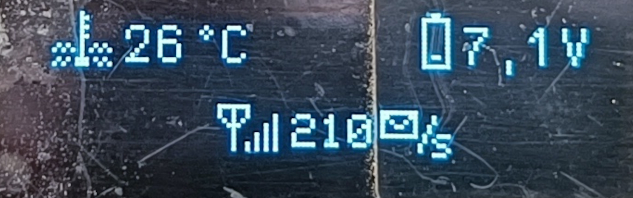
\includegraphics[width=1\textwidth]{fig/car_oled_ok.jpg}
%		\caption{front side}
    \end{subfigure}%
    \hspace{1cm}
    \begin{subfigure}{0.4\textwidth}
    \centering
		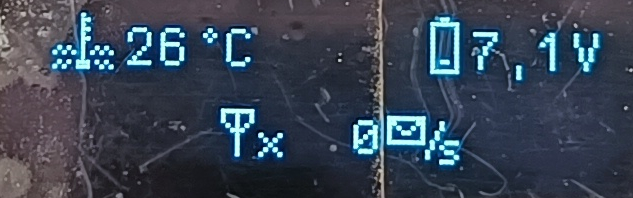
\includegraphics[width=1\textwidth]{fig/car_oled_nosig.jpg}
%		\caption{back side}
    \end{subfigure}
	\caption{OLED display interface in car}
    \label{fig:car_oled}
\end{figure}

\subsection{UART debug prints}
One of the UARTs is reserved for printing debug information. Corresponding pins are available on the pin header under the display; configuration is in section \ref{sub:car_conf}. The behavior is the same as in the transmitter.

The printing is enabled by default after the application start and prints the initialization progress. Afterward, the printing is dependent on the state of the Switch1.

The UART is deinitialized before entering the main control loop if the switch is in the off position or stays initialized otherwise. If debug prints are enabled, the car informs about:
\begin{itemize}
\item LiPo battery voltage and current, VDDA voltage, 5V supply voltage, and BLDC temperature whenever new data is available,
\item file sync, save, write error if SD logging is enabled,
\item switch position changes and push-button presses,
\item no signal state.
\end{itemize}
Debug printing can be enabled or disabled anytime during the application execution.
	\clearpage
	
%!TEX ROOT=main.tex


\part{Results}
\label{chap:results}
\section{Overall}
The built RC system was successfully tested in real-life conditions. The car behaves as expected from an RC car. The connection between the transmitter and the car is quickly established, even though the antenna is usually hidden under the plastic shell. The driving works flawlessly; the control is responsive and smooth. Trimming encoders can correct any misbehavior, for example, small steering to one side.

Suppose the signal is lost and no command arrives in \SI{250}{\ms} from the last one. In that case, the dedicated safety-timer resets actuators to their neutral position. The vehicle comes to a slow stop and waits until another command packet is successfully received.

Extra features such as OLED status display with interactive indicators also work as expected and wirelessly provide the user with additional information about the RC car.

Data logging to the SD card is operational, too, making it possible to record driving data and analyze them afterward. An example of the graphed output data is in the section below in figure \ref{fig:sd_speed}.

The battery life was not measured as it depends on a lot of factors. However, during the testing, the car was able to drive for about an hour. The battery life of the transmitter could not even be estimated because the battery hardly needed to be charged.

Furthermore, two experiments were realized to obtain maximum speed and communication range.

\section{Speed}
The car's maximum speed was tested in Ladronka park on a flat asphalt cycle path. The speed was measured by GPS and consisted of three test runs. An Honor 9 smartphone running GPS speedometer app DigiHUD was taped to the chassis. Before each run, the app's statistics were reset.

The car accelerated quickly and drove in a straight line with the full throttle until it stopped accelerating visually. Then the throttle was released, and the car performed a U-turn and began accelerating again. This process was repeated at least two times in each run.

Data logging to the SD card was enabled for all three test runs to monitor battery voltage, as the motor's maximum speed depends on its supply voltage. Measured data from the last run are graphed in figure \ref{fig:sd_speed}. The test scheme described above is clearly visible - negative peaks in \textit{'STEER'} data paired with positive peaks in \textit{'GYRO\_Z'} data represent U-turns; saturated \textit{'THRTL'} with \textit{'VOLTAGE'} drops and \textit{'CURRENT'} peaks represent straight-line accelerations.
\begin{figure}[h]
\centering
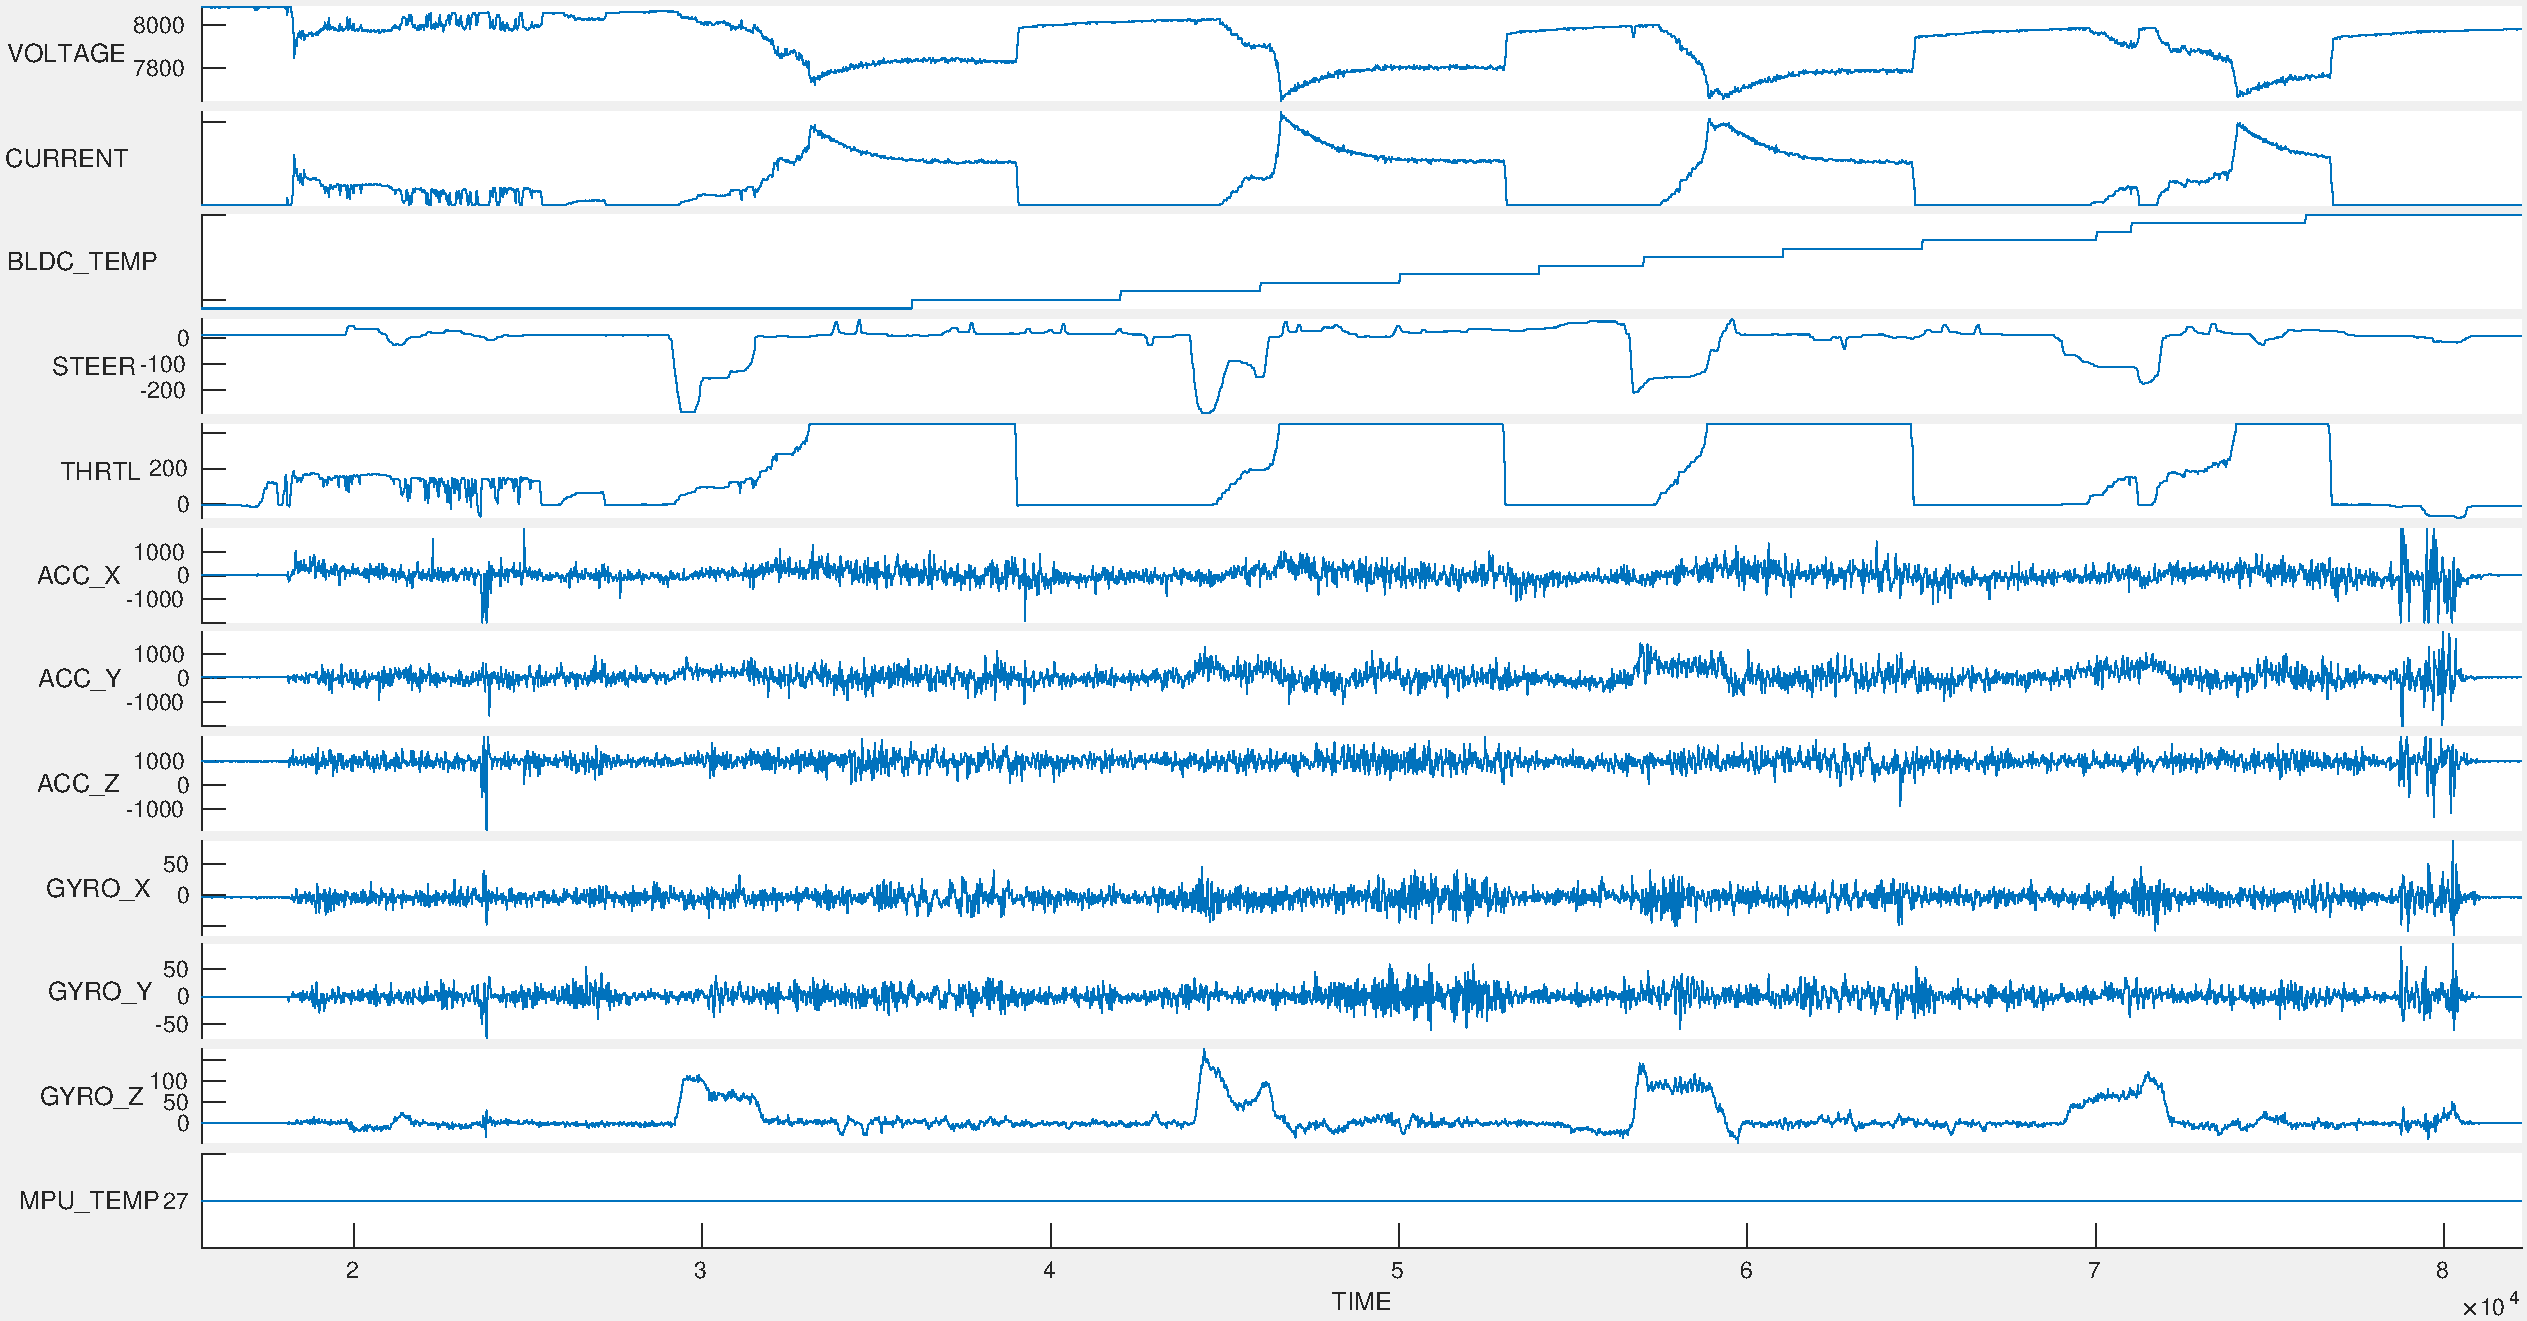
\includegraphics[width=1\linewidth]{fig/run3.pdf}
\caption{Data from last speed-test run}
\label{fig:sd_speed}
\end{figure}

Although the battery voltage dropped by approximately \SI{0.1}{\V} between runs, during all three of them, the car reached a maximum speed of \SI{35}{\km\per\hour}. Photos of the results of the runs are shown in figure \ref{fig:speed}.
\begin{figure}[h]
    \centering
    \begin{subfigure}{0.3\textwidth}
    \centering
        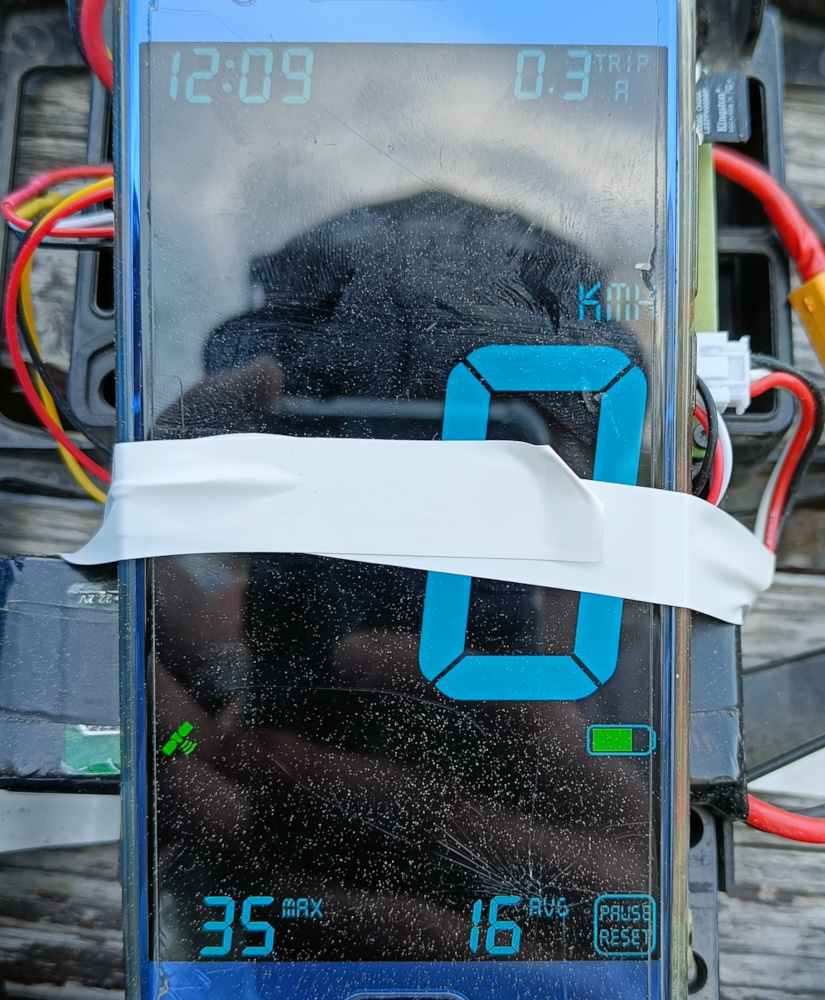
\includegraphics[width=1\textwidth]{fig/speed_run1.jpg}
		\caption{test run 1}
    \end{subfigure}%
    \hspace{0.2cm}
    \begin{subfigure}{0.3\textwidth}
    \centering
		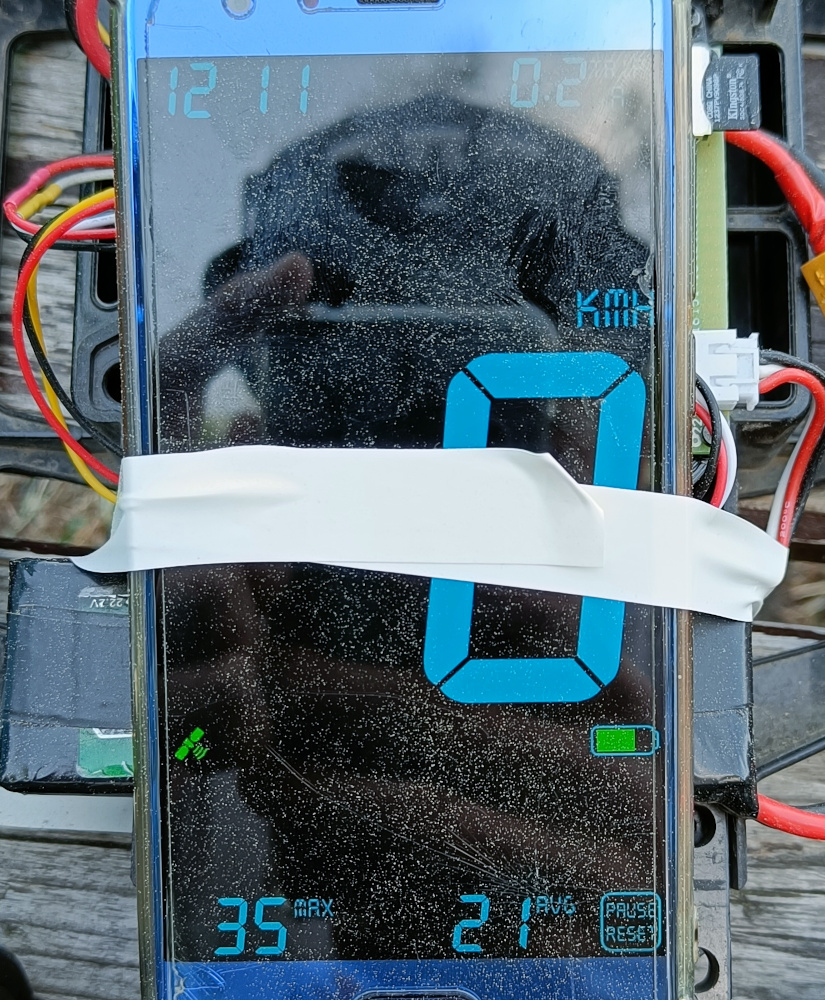
\includegraphics[width=1\textwidth]{fig/speed_run2.jpg}
		\caption{test run 2}
    \end{subfigure}
    \hspace{0.2cm}
    \begin{subfigure}{0.3\textwidth}
    \centering
		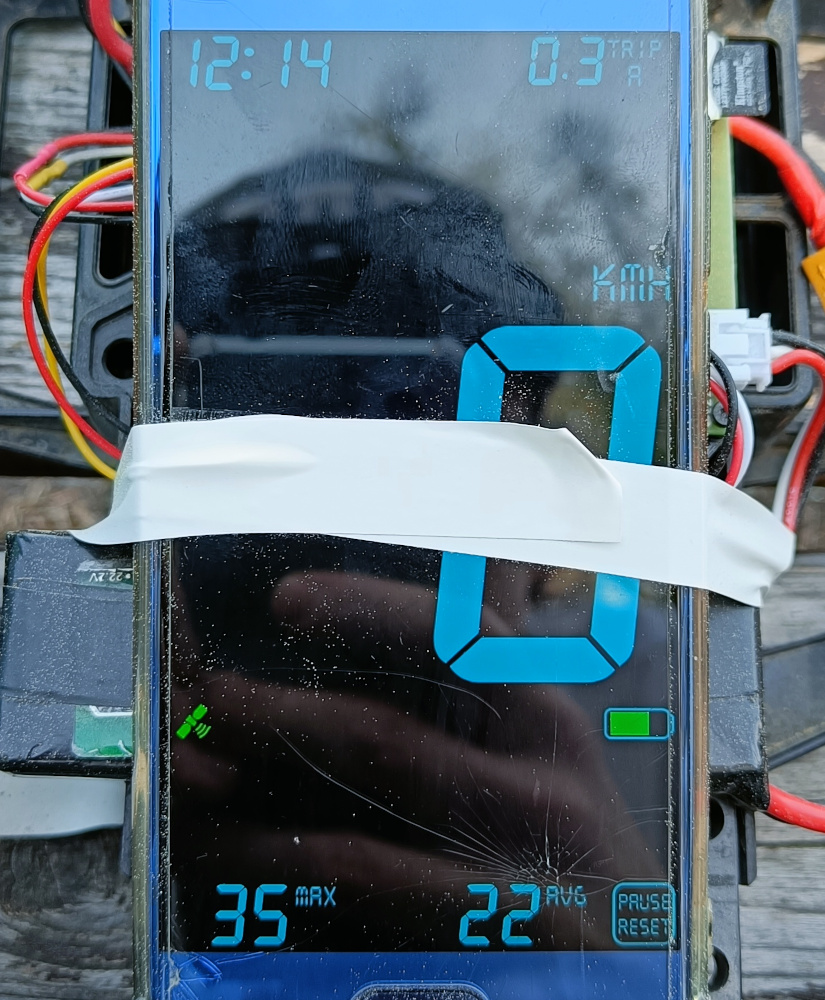
\includegraphics[width=1\textwidth]{fig/speed_run3.jpg}
		\caption{test run 3}
    \end{subfigure}
	\caption{Results of the speed test}
    \label{fig:speed}
\end{figure}

\section{Range}
The range test was also performed in Ladronka park. The test is mainly informative since the car is barely visible at about \SI{250}{\m}. The expected maximum range given by used communication modules was \SI{800}{\m}; therefore, the distance was calculated from GPS coordinates.

The test utilized the vehicle's signal loss detection feature. The transmitter was configured to send the steering command to keep the front wheels turned. The signal loss was easily recognizable since the signal loss detection feature resets the motor and straightens the servo. Both antennas were in a vertical position during the test for the best signal reception.

First, coordinates of the transmitter's initial position were acquired. Then the chassis was moved in a straight direction to keep the transmitter in sight until the signal began to fade.

After \SI{375}{\m}, the servo started to straighten occasionally, indicating that no command packet was received within \SI{250}{\ms} from the last one. Even though the safety-timer sometimes reset the car, it was still controllable.

After \SI{603}{\m} from the initial position, the signal suffered frequent outages. The car was in a 'no signal' state more than 50\% of the time, making the control difficult.

The maximum range was measured at \SI{763}{\m}. At this distance, the signal was not completely lost. Infrequently, the command packet was successfully received, but the car remained in a 'no signal' state most of the time, making the control almost impossible.
\begin{figure}[h]
\centering
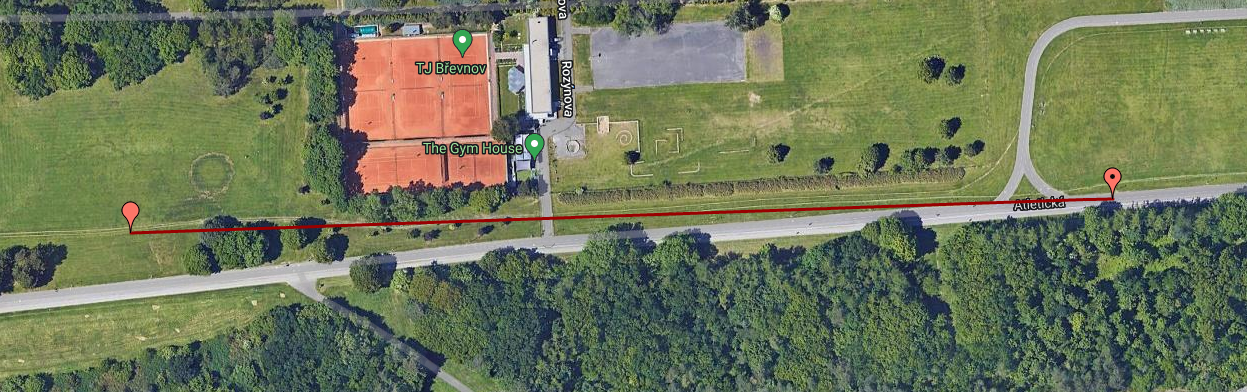
\includegraphics[width=0.9\linewidth]{fig/control_range.png}
\caption{Control distance}
\label{fig:control_range}
\end{figure}

GPS coordinates along with the calculated distance from the initial position are in table \ref{tab:gps_dist}. The measured control distance is visualized in figure \ref{fig:control_range}. 
\begin{table}[h]
   \renewcommand{\arraystretch}{1.1}
   \centering
    \caption{GPS coordinates and distances from the initial position}\label{tab:gps_dist}   
    \begin{tabular}{c c c}
       \noalign{\hrule height 1.1pt}\noalign{\smallskip}
	    & \bfseries GPS coordinates & \bfseries Calculated distance\\[0.2em]
	\noalign{\hrule height 1.1pt}\noalign{\smallskip}     
initial position		& 50.0792036N, 14.3716383E	& -- \\
occasional outages	& 50.0790850N, 14.3663733E	& \SI{375.9}{\m} \\
frequent outages		& 50.0793289N, 14.3631853E	& \SI{603.3}{\m} \\
signal 'lost'		& 50.0794572N, 14.3609497E	& \SI{763.2}{\m} \\
       \noalign{\smallskip}\noalign{\hrule height 1.1pt}
    \end{tabular}
\end{table} 
	\clearpage
	
%!TEX ROOT=main.tex


\part{Conclusion}
\label{chap:conclusion}
The thesis aimed to utilize the STM32 microcontrollers to develop and control an RC car. STM32 families of microcontrollers were summarized, and their architecture and the most commonly used peripherals were briefly described.

The whole system was developed from scratch, aside from the chassis and other plastic parts. It utilizes readily available parts, including an RC servo and BLDC motor with the controller, sensor boards, and modules. These functional blocks were introduced, and their purpose and actual use were explained. Since it is an RC car, meaning 'Radio controlled', the control transmitter was developed as well.

A custom control board was designed for both platforms. The car's control board is made on a perfboard and consists primarily of modules and connectors. This approach is simple, quick, flexible, and certainly sufficient for the use case. However, space constraints inside the transmitter asked for a custom PCB design that would provide better space utilization. Therefore, the circuit board was designed according to the original, slightly modified to fulfill current needs, and manufactured.

The resulting RC system was to be unconventional in terms of available features. Accordingly, both the transmitter and the car received an OLED display and RGB LED to report the status. In addition, the car is equipped with various sensors. A micro SD card slot is available to record all the data.

After the hardware design, a control software had to be developed. As the software controls real devices in real time, it is primarily interrupt-driven and implemented with an emphasis on speed to guarantee periodic execution of the control loop and thus smooth control of the car. Nevertheless, it is also designed to be user-friendly and encompasses interactive battery voltage and signal strength indicators that should simplify navigation on display along with other icons.

At the end of the thesis, the RC system is tested in real conditions with successful results. Besides the essential RC car functions, all the unconventional functions also proved to work. The control is responsive. The car's top speed is 35km/h, and the maximum controllable range is 375m.

All the schematics, source code, and 3D models are available at a GitHub repository\footnote{\url{https://github.com/lunakiller/project_tamiya}} and on the attached DVD.

Even though the feature is not implemented in the project's current state, microcontroller pins PA11 and PA12 on the car's control board are reserved for the USB peripheral. Therefore, a single-board computer like RaspberryPi running a control software can possibly control the car through the USB, and the chassis can, for example, become a platform for testing autonomy.

The future work can possibly be replacing the commercial ESC controlling the motor with some custom-made solution that would offer a more advanced motor control algorithm. This upgrade would increase the top speed, prolong battery life, and provide the user with more driving data.

Another future step would be replacing the present 6-axis IMU with a 9-axis IMU with an incorporated magnetometer to obtain the precise position in space and utilize those data for control or mapping purposes. One possibility would be to utilize those data to implement 'stability control' to help steer the car in a skid or at high speeds, where the car is tricky to control.
	\clearpage
    
%%%%%%%%%%%%%%%%%%%%%%%%%%%%%%%%%%%%%%%%%%%%%%%%%
%% References
%%%%%%%%%%%%%%%%%%%%%%%%%%%%%%%%%%%%%%%%%%%%%%%%%
    \bibliography{main}
    \bibliographystyle{unsrtnat} %use either 'unsrt', 'IEEEtran' or 'named'
    \clearpage
\end{document_body}
 
%%%%%%%%%%%%%%%%%%%%%%%%%%%%%%%%%%%%%%%%%%%%%%%%%
%% Appendices
%%%%%%%%%%%%%%%%%%%%%%%%%%%%%%%%%%%%%%%%%%%%%%%%% 
\begin{document_appendices}
    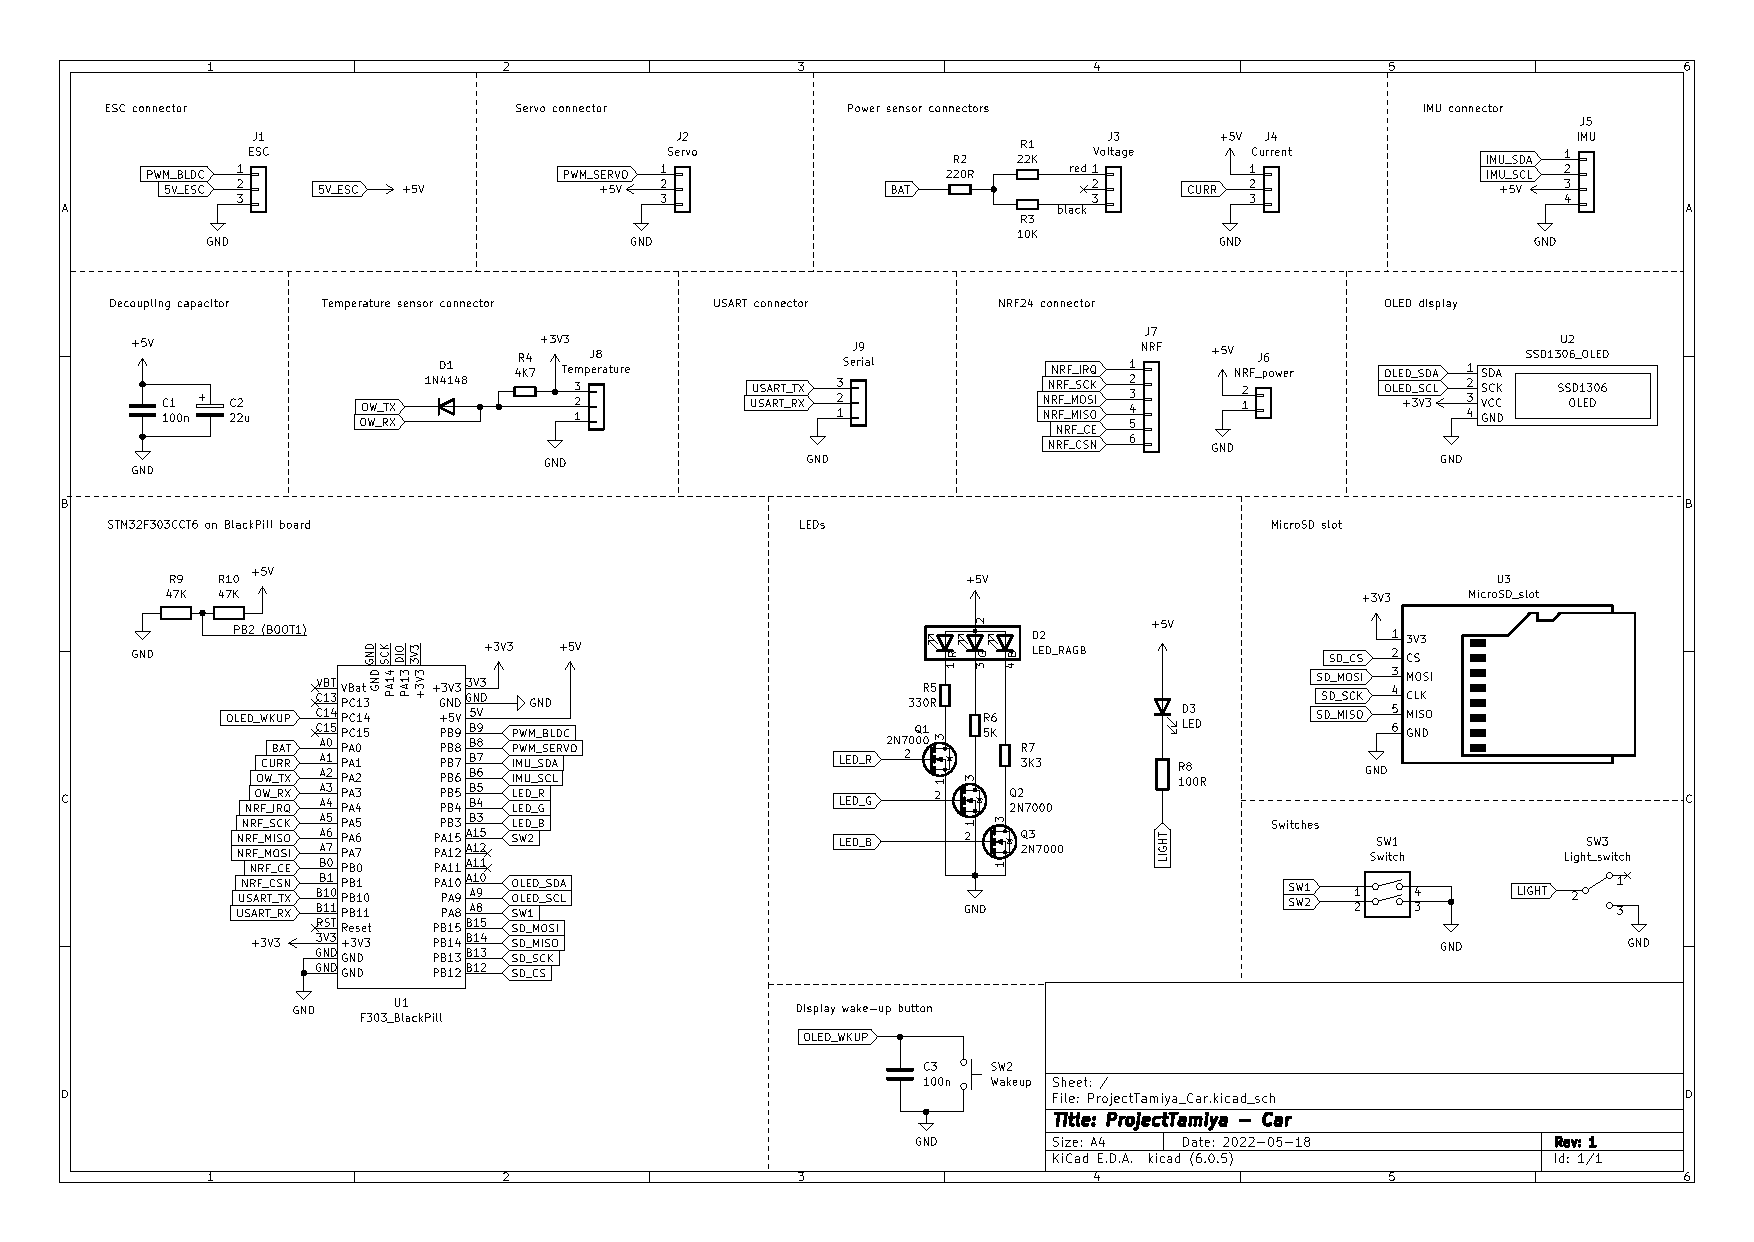
\includepdf[pages=1, angle=90, scale=0.78, offset=0 -45, pagecommand=\appendix{Schematics}]{fig/ProjectTamiya_Car_schematics.pdf}
\newpage
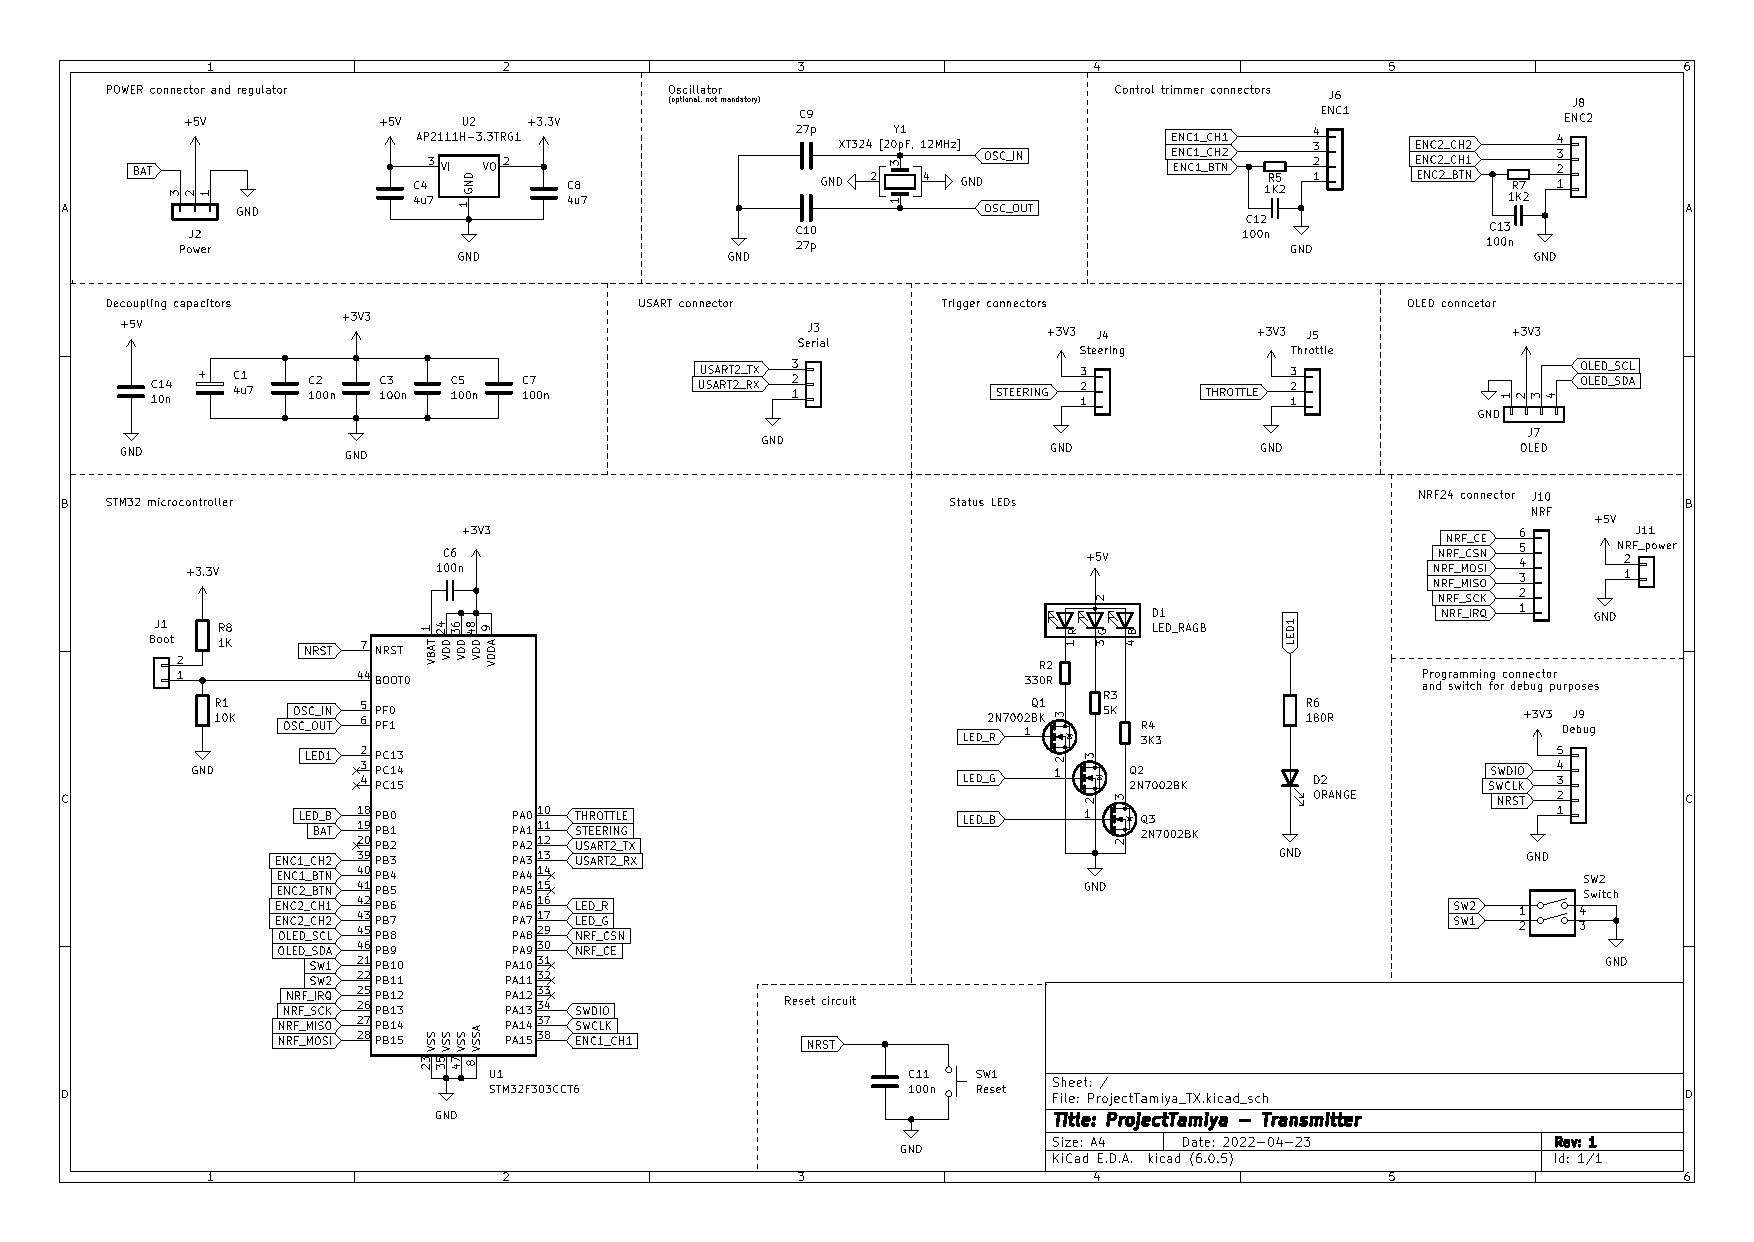
\includepdf[pages=1, angle=90, scale=0.78, offset=0 -20, pagecommand={}]{fig/ProjectTamiya_TX_schematics.pdf}

\newpage
\appendix{Supplementary material}
The attached DVD shares the same file structure as mentioned GitHub repository and is described below. Only the folders have been compressed into zip archives.

\begin{table}[h]
   \renewcommand{\arraystretch}{1.1}
   \centering
%    \caption{ARM Core utilization in STM32 family}
    \label{tab:abbrev}   
    \begin{tabular}{c c}
       \noalign{\hrule height 1.1pt}\noalign{\smallskip}
	   \bfseries File & \bfseries Contents\\[0.2em]
	\noalign{\hrule height 1.1pt}\noalign{\smallskip}  

Software.zip 			& source codes and drivers for both control applications, shared libraries \\
Hardware.zip 			& KiCad schematics and gerber files \\
3D\_printed\_parts.zip	& STL models for 3D printing \\
Logs.zip					& Two example logs in CSV format \\

       \noalign{\smallskip}\noalign{\hrule height 1.1pt}
    \end{tabular}
\end{table} 

\end{document_appendices}
\end{document}
